\documentclass[oneside, ngerman, toc=bibliography,bibliography=totoc,listof=entryprefix, open=right,numbers=noenddot,fontsize=12pt]{scrbook}

% für sabine 14pt setzen

\usepackage{ngerman}
\usepackage[ngerman]{babel}
%\usepackage[german]{hyphenat}
\sloppy 
\usepackage[none]{hyphenat}  % stelle die meist falsche silbentrennung ab

\usepackage[onehalfspacing]{setspace}

\usepackage[T1]{fontenc}
\usepackage[utf8]{inputenc}
\usepackage{cmap}
%\usepackage{bibgerm} % Verwendet deutsche Abkürzungen

\usepackage[a4paper, left= 3cm, right=2cm, top=2.5cm, bottom=2cm, includeheadfoot]{geometry}




\usepackage{booktabs} % Benutze booktabs, um korrekt gesetzte, SCHOENE Tabelle zu erzeugen http://www.math.utah.edu/tex-archive/macros/latex/contrib/booktabs/booktabs.pdf

\usepackage{longtable} % Für Tabellen, die länger als eine Seite sind. Der Seitenumbruch erfolgt dann automatisch. Bsp.: Glossar

\usepackage{times} % andere schrift

% jpeg png etc. erlauben
\usepackage{graphicx}
\usepackage{epsfig}
\usepackage{graphics}
%\usepackage{color}
\usepackage{xcolor} 
% Komfortableres Tabellen-Paket
\usepackage{tabularx}
\usepackage{tabu}
% Ermöglicht mehrere Bilder in einer floatenden Figure-Umgebung
%\usepackage{subfig}
%\usepackage{ulem}
%\usepackage{csquotes}



% Erlauben von urls
\usepackage{url}
\usepackage{hyperref}
\usepackage{letterspace}	% For extended line spacing on title page

%\usepackage[overload]{textcase}
% \usepackage{listings}
 
%python Pygments und -shell-escape
% \usepackage{minted}
\usepackage[framemethod=default]{mdframed}

\newcommand{\autor}{Jens Kapitza}
\newcommand{\titel}{SciServer -- Entwicklung einer Serversoftware zur Verwaltung von wissenschaftlichen Daten}
\newcommand{\ort}{Duisburg}
\newcommand{\einreichung}{20.10.2015}
\newcommand{\matrikelnr}{2242777}
\newcommand{\studiengang}{Angewandte Informatik}
\newcommand{\arbeit}{Masterarbeit}
\newcommand{\erstpruefer}{Prof.\ Jens Krüger}
\newcommand{\zweitpruefer}{Prof.\ Torben Weis}
\newcommand{\abschluss}{Master of Science (M. Sc.)}

% Klickbare Links innerhalb des PDFs
\hypersetup{ pdftitle={SciServer}, pdfauthor={\autor{}}, pdfsubject={\arbeit{}}, colorlinks=false, breaklinks=true }



% andere schrift beim zitieren
\AtBeginEnvironment{quote}{\setlength{\textwidth}{0.7\textwidth}\itshape\small}

\newcommand\chapmd[2]{\begin{mdframed}[%
		rightline=false,leftline=false,topline=false,bottomline=false,frametitlerule=false,
		userdefinedwidth=\textwidth,frametitlealignment=\flushright, %frametitlebackgroundcolor=gray!5,
		frametitlerulecolor=black,frametitle={\small #1}]
		\flushright{} \footnotesize{} #2
	\end{mdframed}}

% Style Minted
%\usemintedstyle{default}
%\newminted{java}{linenos=true, numbersep=5pt,fontsize=\footnotesize,texcl=true}
%\newminted{xml}{linenos=true,numbersep=5pt,fontsize=\footnotesize,texcl=true}
%\newminted{shell}{linenos=true,numbersep=5pt,fontsize=\footnotesize,texcl=true}

\usepackage[nonumberlist,nopostdot]{glossaries}
\makeglossaries
\usepackage[xindy]{imakeidx}
\makeindex



\usepackage{xparse}
\DeclareDocumentCommand{\newdualentry}{ O{} O{} m m m m } {
    \newglossaryentry{gls-#3}{name={#5},text={#5\glsadd{#3}}, description={#6},#1}
    
    \newacronym[see={[Glossary:]{gls-#3}},#2]{#3}{#4}{#5\glsadd{gls-#3}}
}

\begin{document}


\newdualentry{dms} % label
{DMS}            % abbreviation
{Datenmanagementsystem}  % long form
{System zum Verwalten von Dateien, in dem auch gesucht werden kann.} % description
 
\newdualentry{p2p} % label
{P2P}            % abbreviation
{Peer-to-Peer}  % long form
{Kommunikationsmodell, in dem jeder Teilnehmer mit jedem anderen reden kann.} % description
 
\newdualentry{nfs} % label
{NFS}            % abbreviation
{Network File System}  % long form
{Bei Linux gleichnamiger Dienst, generell ist ein Netzwerkdienst gemeint, welcher sein Dateisystem über einen Computer hinweg zur Verfügung stellt.} % description
 
\newdualentry{cifs} % label
{CIFS}            % abbreviation
{Common Internet File System}  % long form
{Netzwerk Kommunikationsprotokoll, unter Windows und durch Samba unter Linux bereitgestellter Dienst zum Datenaustausch zwischen Computern.} % description

\newdualentry{ads} % label
{ADS}            % abbreviation
{alternative data streams}  % long form
{Windows Funktion zur Datenspeicherung innerhalb einer Datei} % description
 
\newdualentry{rf} % label
{RF}            % abbreviation
{resource forks}  % long form
{Eine Technologie, die von Apple verwendet wurde, zur Datenspeicherung innerhalb einer Datei.} % description

\newdualentry{lvm} % label
{LVM}            % abbreviation
{Logical-Volume-Manager}  % long form
{Ein LVM, bietet einen virtuellen Zusammenschluss mehrerer Festplatten zu einem logischen Laufwerk. } % description



\newdualentry{rpc} % label
{RPC}            % abbreviation
{Remote Procedure Call}  % long form
{Aufruf einer fernen Prozedur} % description



\newdualentry{nat} % label
{NAT}            % abbreviation
{Network Address Translation}  % long form
{Verfahren zum Ersetzen der Adressinformationen in IP Datenpaketen} % description


\newdualentry{jms} % label
{JMS}            % abbreviation
{Java Message Service}  % long form
{Bibliothek zum Kommunizieren durch Nachrichtenaustausch. } % description
 
 \newdualentry{pae} % label
 {PAE}            % abbreviation
 {Physical Address Extension}  % long form
 {Erweiterung der Adressierung in 32 Bit Architektur} % description
 
 
\newdualentry{cdi} % label
{CDI}            % abbreviation
{Contexts and Dependency Injection}  % long form
{Aus Java EE, Möglichkeit zur Auflösung von Objektabhängigkeiten zur Laufzeit sowie Verwaltung von Lebenszyklen verwalteter Objekte innerhalb einer Anwendung.} % description

\newdualentry{jpa} % label
{JPA}            % abbreviation
{Java Persistence API}  % long form
{API in Java zur Verwendung einer Datenbank, diese API beinhaltet auch eine \acrshort{orm} Abbildung von Klassen auf Tabellen der Datenbank.} % description
 
\newdualentry{orm} % label
{ORM}            % abbreviation
{Object-Relational Mapping}  % long form
{Bidirektionale Abbildung der Spalteninformationen einer Datenbank in Eigenschaften eines Objektes.} % description

\newdualentry{tls} % label
{TLS}            % abbreviation
{Transport Layer Security}  % long form
{Verschlüsselung durch Zertifikate, häufige Verwendung bei HTTPS, SMTPS, FTPS. Sollte nicht mit SFTP verwechselt werden, welches ein anderes Verfahren nutzt (Schlagwort: SSH).} % description
 

\newdualentry{ide} % label
{IDE}            % abbreviation
{Integrierte Entwicklungsumgebung}  % long form
{Eine IDE erlaubt das einfachere Schreiben von Quellcode und unterstützt verschiedene Tools, die das Arbeiten z. B. mit Datenbanken vereinfachen.} % description




\newdualentry{ttl} % label
{TTL}            % abbreviation
{Time to live}  % long form
{Lebenszeit, z. B. für ein Verwerfen eines Paketes im Netzwerk.} % description


 
\newdualentry{fqdn} % label
{FQDN}            % abbreviation
{Fully Qualified Domain Name}  % long form
{Absoluter vollständiger Domainname eines Computers.} % description
  
 
 
 
 \newdualentry{stun} % label
 {STUN}            % abbreviation
 {Session Traversal Utilities for NAT}  % long form
 {Möglichkeit zum Erkennen der externen Verbindungsparameter sowie den \acrshort{nat} Firewall-Typen für anfragende Geräte.} % description
 
  
 
 \newdualentry{acc} % label
 {ACC}            % abbreviation
 {Application Client Container}  % long form
 {Spezielle Form eines Clients, der komplett vom Anwendungsserver abhängig ist.} % description
 
 \newdualentry{KEY} % label
 {ABBR}            % abbreviation
 {LONG}  % long form
 {DESC} % description
 
 
 
 

\author{\autor{}}
\title{\titel{}}
\date{\einreichung{}}


\frontmatter
\pagenumbering{Roman}

\begin{titlepage}
%\enlargethispage{2cm}

\includegraphics[width=6cm]{uni-logo.pdf}\\
\\[1cm] 
\vspace*{4cm}\noindent
\textls[70]{ \Large{\sf{\MakeTextUppercase{\arbeit{}}}}}\\
\huge{\sf{ \textbf{\titel{}}}}\\[1cm]
\textls[70]{\Large{\sf{von \autor{} (Matrikel-Nr.: \matrikelnr{})}}}%[6cm]

\vspace*{\fill}
\normalsize
\begin{center}
\begin{tabularx}{0.9\textwidth}{Xl}
      & Erstprüfer: \erstpruefer{}\\
      & Zweitprüfer: \zweitpruefer{}
\end{tabularx}
\end{center}

\vspace*{1cm}
Eine Abschlussarbeit im Studiengang \studiengang{}, vorgelegt der Abteilung Informatik und Angewandte Kognitionswissenschaft an der Universität Duisburg-Essen zur Erlangung des akademischen Grades \abschluss{}.
\end{titlepage}


\cleardoublepage
\vspace*{\fill}
\section*{Zusammenfassung}


Zeitgemäße Datenspeicherung erfordert auch ein einfaches und effizientes Suchen über die gespeicherten Daten. Da Weboberflächen immer beliebter werden, gerade durch die mobilen Endgeräte, wird im Rahmen dieser Masterarbeit ein Such- und Benachrichtigungssystem entwickelt. Die Anwendung verwendet dabei einen \acrfull{p2p} Ansatz und versucht möglichst viele externe Dienste wiederzuverwenden. Wegen der enormen Dateigröße ist ein direktes Arbeiten und Analysieren der Dateien nicht sofort möglich. Berechnungen wie die Prüfsumme nehmen viel Zeit in Anspruch, und sollen möglichst daher zwischengespeichert werden, um im Fall eines Datenabgleiches nicht ständig neu zu berechnen.\\[2cm]
{\bf Schlüsselbegriffe:} Java, Maven, \acrfull{p2p}, Napster, Nachrichten basierte Kommunikation, Watchservice, Dateibenachrichtigungen, Bigdata, erweiterte Attribute, Tagging, Verschlagwortung, Suchen und Filtern, 
\vspace*{\fill}
\cleardoublepage


\vspace*{\fill}

\noindent Hiermit erkläre ich, dass ich die Masterarbeit eigenständig verfasst und keine anderen
als die angegebenen Quellen und Hilfsmittel benutzt habe.
Alle Stellen der Arbeit, die wörtlich oder sinngemäß aus \mbox{Veröffentlichungen} oder aus anderweitigen
fremden Äußerungen entnommen wurden, sind als solche kenntlich gemacht.

\vspace{30mm}


\begin{tabularx}{\linewidth}{Xr}\cline{2-2}
& \ort{}, \einreichung{}, \autor{}
\end{tabularx}


\cleardoublepage
\vspace*{3cm}
\begin{quote}\Large
\centering
    Wer nicht danke sagen kann,\\wird irgendwann vergeblich bitten.\\
    {\small -- Fred Ammon,  \verb|http://www.aphorismen.de| }
\end{quote}
\vspace*{3cm}
\noindent
Danke für eure Unterstützung an Freunde und Familie. \\ \bigskip \\
Besonderer Dank gilt: \\

Ralf Marquis und Sabine Budde-Marquis,

Sarah Rzeha,

Patrick Litzbarski und 

Günter und Heidi Kapitza

\pagebreak
%\glsaddall


\tableofcontents{}

\mainmatter{}


\chapter{Einleitung}
\label{chap:einleitung}
\chapmd{Facebookseite der MythBusters (26.09.2013)}{,,Remember kids, the only difference between screwing around and science is writing it down.''}

Zeitgemäße Datenspeicherung erfordert auch ein einfaches und effizientes Suchen über die gespeicherten Daten. Da Weboberflächen immer beliebter werden, gerade durch die mobilen Endgeräte, wird im Rahmen dieser Masterarbeit ein Such- und Benachrichtigungssystem entwickelt. Ziel soll es sein, einen Datenbestand zur effizienten Suche einfach aufzubereiten und Änderungen an den bestehenden Daten oder neu erstellten Dokumenten zu überwachen.

Informationen über die Dateien werden in einer separaten Datenbank gespeichert und mit Hilfe eines Menschen ergänzt. Ergänzungen können dabei Schlagworte oder Schlüssel-Wert-Paare sein. Über die gewonnenen Informationen werden Suchanfragen formuliert und die Ergebnisse dem Benutzer zur Weiterverarbeitung angezeigt. Auf der Anzeige sind Operationen wie Vorfilterung durch separate Prozesse oder weiteren Ergänzungen möglich.

Bei den Benachrichtigungen handelt es sich um E-Mails mit Informationen über Dateien, die registrierten Benutzern gesendet werden. Das System erlaubt E-Mail-Antworten zur betroffenen Datei und kann so bereits erste ergänzende Informationen zur Datei aufnehmen.


\section{Beschreibung des Problems}


\begin{quote}
The focus of this project is to develop a dataset management system for scientific datasets such as regular tensor, vector and scalar fields, meshes, and other unstructured data.
Most research groups store their datasets as simple files in a directory structure on their file servers. This makes it hard to assign properties to the files to efficiently search them. While platform specific solutions exist these are usually not exposed in a platform independent way over the network.
In this thesis a platform independent web-based solution is to be developed to efficiently, store, access, replicate, and process these datasets. In this system scalability is a major concern as scientific datasets may easily grow to dozens of terabytes per dataset. 
\end{quote}


Der Auszug der \href{http://hpc.uni-due.de/theses.html}{Lehrstuhlwebseite} vom 20.04.2015 um 12:00 Uhr beschäftigt sich mit dem Problem der Verwaltung wissenschaftlicher, unstrukturierter Daten. Dabei wird die Idee skizziert, eine webbasierte Plattform für die Suche und den Zugriff auf Datenspeicher zu erstellen. Informationen einer Datei sollen dabei von dem  \acrfull{dms} verwaltet werden. Das \acrshort{dms} bereitet die gewonnenen Informationen auf und ermöglicht eine einfache Suche.

\section{Ziel der Arbeit}
Im Rahmen der Arbeit wird ein  \acrfull{p2p}  basiertes \acrshort{dms} entwickelt. Durch den \acrshort{p2p}-Gedanken wird nicht nur eine horizontale Skalierung ermöglicht, sondern auch das Anbinden weiterer Dienste. Mailserver oder Datenspeicher (\acrfull{nfs}, \acrfull{cifs}, \ldots) werden in dem System durch passende Proxy dargestellt. Die Stellvertreter dieser Dienste bilden eine einheitliche Kommunikationsebene \cite{coulouris2002verteilte} und erlauben das Fokussieren auf die Kernfunktion. Eine webbasierte Anwendung stellt dem Anwender die Suchoberfläche bereit und ermöglicht ihm dadurch das Interagieren.

Wird die Anwendung in die definierten Kategorien eingeordnet, so folgt diese dem Ansatz einer Vermittler basierten Lösung \cite{backx2002comparison}. Das Problem des Bootstrapping wird hier mit Hilfe des Vermittlers gelöst (vgl. { Napster} \cite{mahlmann2007peer}) \cite{4144906}. Bei diesem Ansatz ist der Vermittler jedoch ein ,,single point of failure'', der dem \acrshort{p2p}-Gedanken widerspricht. 

Der Vermittler sammelt alle Informationen, wie Pfade oder Zeitstempel, zu den einzelnen Dateien ein und speichert diese durch geeignete Peers ab. Die speichernden Peers stellen Suchmöglichkeiten über bestimmte Informationen zur Verfügung und senden das Ergebnis durch den Vermittler zurück.
Suchanfrage-Ergebnisse werden durch die Interaktion mit dem Anwender verbessert, die mit weiteren Eingaben die Abfragemöglichkeiten erweitern.
Beispielsweise wird beim ,,sozial tagging'' mit Schlagwörtern eine Struktur erzeugt \cite{gaiser2008good}.
Der verfolgte Ansatz speichert die Dateien nicht beim Vermittler, sondern lässt sich die fertigen Analysen durch geeignete Peers übermitteln.

Neben dem Bereitstellen der Such-Weboberfläche ist die Dateisynchronisation durch den Vermittler koordiniert und erinnert an Funktionen wie Server zu Server Kommunikation in FTP \cite{rfc959}.

Durch eine Brücke ist es möglich, einen ,,super-peer'' zu erstellen \cite{yang2003designing}. Der Vermittler interagiert in einem Netzwert von Vermittlern und kann Informationen bereitstellen oder auch empfangen.

\section{Themenabgrenzung / Restriktion}
Im Rahmen der Arbeit bleibt der Aspekt der Relevanzbeurteilung unberücksichtigt. Es handelt sich bei den Suchergebnissen um nicht gewichtete Mengen. Nach Aufgabenstellung wird auch die Informationsextraktion mit Tools wie \href{http://tika.apache.org/}{Apache Tika} oder  \href{http://pdfbox.apache.org/}{Apache PDFBox} nicht weiter verfolgt, da die unstrukturierten Daten entsprechend der Aufgabenstellung nicht durch {Magic-Numbers bzw. MIME-Types} zu erkennen sein sollen. 


\section{Analyse des IST-Zustandes}\label{sec:ist}

Entsprechend der Aufgabenstellung müssen mindestens drei Szenarien aus Anwendersicht unterstützt werden:
\begin{itemize}
	\item Das Suchen nach Dateien über einen Datenbestand.
	\item Das Zugreifen auf die Daten.
	\item Das Synchronisieren der Daten, welches als Kombination der beiden zuvor genannten aufgefasst werden kann.
\end{itemize}

Bevor auf die einzelnen Szenarien im Detail eingegangen wird, wird zunächst durch die Abbildung \ref{fig:ist-struktur} schematisch die aktuelle Systemarchitektur verdeutlicht. Zwei Universitäten kommunizieren über einen Server (Cloud Dienst, \ldots). Dadurch ist es Lehrstühlen möglich, Daten untereinander auszutauschen. Dieser Austausch erfordert aber das Nutzen anderer Dienste oder ist nur auf kleine Daten beschränkt. Um effizienter Daten auszutauschen und nicht mehrere Stunden auf den Transfer zu warten, muss das Suchen über nicht vorhandene Daten ermöglicht werden.

\begin{figure}[htbp] 
    \centering
    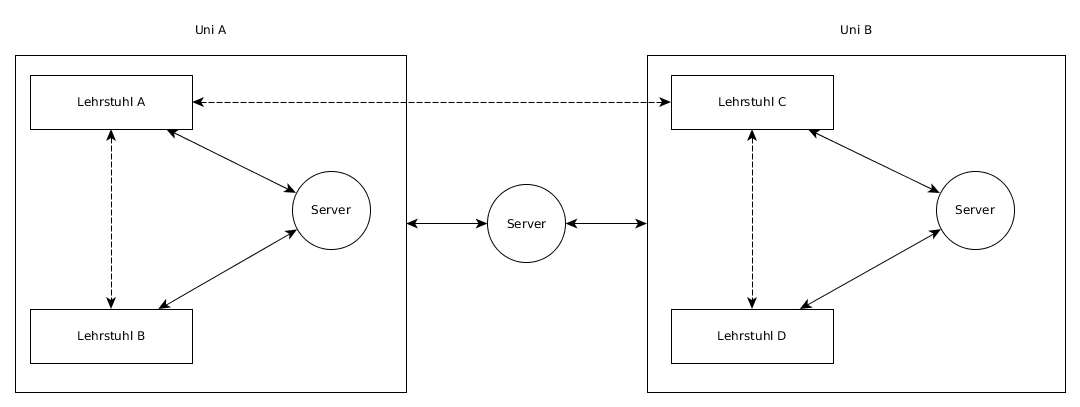
\includegraphics[width=\textwidth]{Masterarbeit_Bilder/Lehrstuhl_Datentausch_extern.png}
    \caption{Schematischer Aufbau des Universitätsnetzwerkes}
    \label{fig:ist-struktur}
\end{figure}    

Das Problem  lässt sich von einer ,,Uni'' auf einen Lehrstuhl reduzieren, wie  die Abbildung \ref{fig:ist-struktur2} schematisch aufzeigt.
Auf den als ,,Server'' gekennzeichneten Objekten laufen diverse Dienste (Datenspeicherung, E-Mail).

Schaut man sich in der Abbildung einen Arbeitsbereich an, so findet man in diesem auch Endgeräte, die über unterschiedliche Protokolle (HTTP, SMTP, IMAP, \ldots) mit den Server kommunizieren.

\begin{figure}[htbp] 
	\centering
	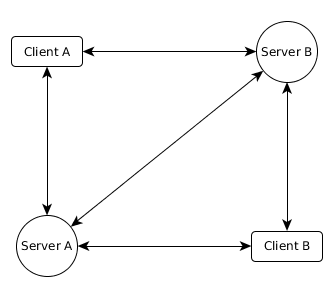
\includegraphics[width=0.8\textwidth]{Masterarbeit_Bilder/Lehrstuhl_Datentausch_intern.png}
	\caption{Schematischer Aufbau eines Lehrstuhls}
	\label{fig:ist-struktur2}
\end{figure}  

 Ein Server wie in Abbildung \ref{fig:ist-server} stellt Dienste zur Verfügung und unterscheidet sich von einem Endgerät wie in Abbildung \ref{fig:ist-endgeraet} lediglich durch die Dienste bzw. Programme, die auf dem Gerät laufen. Ein Server aus traditioneller Sicht ist ein gegen den Ausfall besser abgesicherter Computer. Aus heutiger Sicht lassen sich bezüglich der Leistung für die meisten Anwendungen kaum Unterschiede feststellen.
 
\begin{figure}[htbp] 
	\centering 
	\begin{minipage}{.5\textwidth}
	\begin{tabular}{|p{.9\textwidth}|}
		\hline
Server\\ \hline\hline
\\
NFS | SMB| Appeltalk | \ldots \\ \hline
Betriebssystem \\ \hline
Netzwerk (TCP /IP) \\ \hline
	\end{tabular}
	 
	\caption{Server}
	\label{fig:ist-server}
\end{minipage}%
\begin{minipage}{.5\textwidth}
	\begin{tabular}{|p{.9\textwidth}|}
 		\hline
		Client \\\hline\hline
		Browser \\ \hline
		Netzwerklaufwerk | \ldots \\ \hline
		Betriebssystem \\ \hline
		Netzwerk (TCP /IP) \\ \hline
	\end{tabular}
	\caption{Endgerät}
	\label{fig:ist-endgeraet}
\end{minipage}%
\end{figure}   

Zu den bekanntesten Betriebssystemen gehören Linux (Fedora, Debian, \ldots), Windows oder Mac OS. Zur Vereinfachung beziehen sich die Begriffe  \acrshort{nfs}, Web-Browser, Dateisystem und Dateimanager auf die jeweiligen vom Betriebssystem als Standard genutzten Anwendungen.

Für die nachfolgenden Szenarien wird die Konfiguration wie in Abbildung \ref{fig:ist-struktur2} vorausgesetzt, bei der auf einem von Anwendern bedienten Endgerät ein Netzwerklaufwerk oder eine Festplatte verbunden ist. Es gibt einen oder mehrere Anwender, deren Prozesse vom Server oder Betriebssystem des Endgerät koordiniert werden müssen. Anwendern ist neben einem Benutzernamen auch eine E-Mail-Adresse zugeordnet, unter denen diese erreichbar sind.

Server können zwar als Endgerät agieren, sprechen jedoch meist mehr Protokolle, um untereinander Informationen auszutauschen. Da die Server meist durch einen Administrator fest definierten Abläufen folgen, wird im weiteren Verlauf nicht mehr auf diese eingegangen.


\subsection*{Suche über den Datenbestand}
Es wird im entsprechenden Suchfeld des Dateimanagers nach einem Dateinamen oder bekannten Schlagwort gesucht. Anschließend wird die Ergebnisliste ausgewertet.

\bigskip
Folgende Probleme können anhand des Szenarios festgehalten werden:
\begin{itemize}
	\item Lange Suchzeiten, wenn keine Datenbank mit Indizierung verwendet wird.
	\item Kaum Unterstützung bei der Suche, meist keine Verwendung der Verschlagwortung oder nur eingeschränkt nutzbar. 
	\item Benutzerinterfaces unterscheiden sich in der Unterstützung je nach verwendeter Plattform (siehe Kapitel \ref{chap:techAnal}).
	\item Bei Verwendung von gewissen Attributen gibt es nicht immer passende Unterstützung innerhalb des \acrshort{nfs} oder Dateisystems.
\end{itemize}

\subsection*{Zugriff auf den Datenbestand}
Mit bekanntem Dateinamen kann auf das entsprechende Laufwerk und anschließend auf die gewünschte Datei zugegriffen werden.

\bigskip
Folgende Probleme können anhand des Szenarios festgehalten werden:
\begin{itemize}
	\item Die meisten Unterstützungen, wie direktes Arbeiten auf einer Datei, sind Plattform abhängig.
	\item Bei langen Pfaden wird das Navigieren komplexer.
\end{itemize}


\subsection*{Synchronisation der Daten}
Mindestens zwei Server, die ihren Datenbestand abgleichen wollen, suchen untereinander nach nicht vorhandenen Dateien und übertragen diese gegenseitig.

\bigskip
Folgende Probleme können anhand des Szenarios festgehalten werden:
\begin{itemize}
	\item Sind die Datenspeicher unterschiedlich groß, können Datenbestände auf einem Server von unterschiedlichen Servern stammen.
	\item Sind die Datenspeicher unterschiedlich groß, müssen Datenbestände eines Server ggf. auf mehrere aufgeteilt werden.
	\item Durch unterschiedliche Protokollabläufe in einem heterogenen Netzwerk ist die optimale Geschwindigkeit selten gewährleistet.
\end{itemize}
 
\subsection*{Zusammenfassung}
Die Arbeitsumgebung umfasst als Datenspeicher neben RAID-Systemen auf Servern auch Technologien  wie USB,  \acrshort{cifs} oder \acrshort{nfs}.
Auf den Computern liegen verschiedene Dateisysteme und Betriebssysteme mit starken Abweichungen in ihrer Funktionalität vor.

Einzige Annahme für die Arbeit ist, dass auf den Endgeräten ein Webbrowser und  E-Mail-Client (mindestens eine Webschnittstelle) bereitgestellt sind.
Die Server können im Gegensatz zu vielen Endgeräten meist einfacher mit weiteren Programmen bestückt werden.

Die Anwender rufen ihre Daten durch die entsprechenden Netzwerklaufwerke ab.
Ein Übertragen der Daten ist wegen der Größe aus Zeitgründen nach Vorgabe nicht akzeptabel. Dem Anwender ist mindestens ein Benutzerkonto mit E-Mail-Adresse zugewiesen.

\bigskip
Es ergeben sich Anforderungen für die Realisierung wie:
\begin{itemize}
\item Zuordnung einer Person zu den diversen Konten an den entsprechenden Servern und Endgeräten
\item Auslesen der Informationen einer Datei unter Beachtung des Dateisystems
\item Zuordnung einer Datei zur entsprechenden Person als Verantwortlicher
\item Anzeigenanpassung und individuelle Unterstützung je nach verwendeter Plattform
\item Übertragung der Dateien zwischen teilnehmenden Computern
\item Benachrichtigung über den Vorgang wie beim Kopieren, Erstellen und Löschen einer Datei
\item Persistente Speicherung aller Informationen zu einer Datei über die vom Dateisystem unterstützten Funktionen hinaus
\item Verlinken der \acrshort{dms}
\item Erkennung doppelter Dateien
\end{itemize}
 


\chapter{Grundlagen und verwandte Ansätze}
\chapmd{Albert Einstein (1879--1955)}{,,So einfach wie möglich. Aber nicht einfacher!''}

In der Einleitung wurden Anforderungen, Annahmen und Umfeld der Anwendung skizziert.
Um das WIE zu klären, wird in diesem Kapitel ein Überblick über diverse Dateisysteme gegeben, Möglichkeiten der Kommunikations-Realisierung gezeigt und bestehende kommerzielle Lösungen einander gegenübergestellt.

\section{Betriebssystem abhängige Verschlagwortung}
In der Einleitung wurde bereits darauf hingewiesen, dass es auf allen Plattformen eine grundlegende Unterstützung für die Verschlagwortung von Dateien gibt. Die Realisierung erfolgt meist durch Verwendung von erweiterten Attributen, die ursprünglich zur Verwaltung der Benutzerrechte verwendet wurden. 

Seit ,,Windows Server 2008'' findet dies auch in einem Domain-Controller statt, zur Abbildung der Rechte in heterogenen Netzen \cite{windowsserver2008}.

Linux kennt erweiterte Attribute, auch um ,,Dateien leichter zu finden'' seit dem Jahr 2004 mit Kernelversion 2.6 \cite{von2006100}. Beschränkungen in der Verwendung sind unter Linux am stärksten, so ist beispielsweise bei Dateisystemen auf Ext2 Basis vor allem die Größe der Schlüssel-Wert-Paare entscheidend. Im Fehlerfall kann eine Meldung wie

\begin{quote}
attr\_set: Auf dem Gerät ist kein Speicherplatz mehr verfügbar
\end{quote}

auftreten. Die Möglichkeiten der Speicherung innerhalb einer INODE der Datei ist in Linux daher begrenzt \cite{kernelwiki}.

Durch eine geeignete Abstraktion ist mit Einschränkungen dennoch eine Betriebssystem übergreifende Lösung realisierbar. So zeigt das Samba-Team mit ihrer Implementierung des Windows Netzwerk Dienstes unter Linux. Die Entwickler weisen jedoch auch auf die Limitierungen in den Dateisystemen auf POSIX Systemen hin  \cite{smb}.

Windows und OS X besitzen eine bessere Unterstützung der ,,erweiterten Attribute''. Die Technologien dahinter heißen \acrfull{ads} bzw.  \acrfull{rf},  um Anhänge zu einer Datei zu speichern \cite{surendorf2010mac}.

OS X besitzt zudem mit HFS+ ein Dateisystem, welches erweiterte Attribute von Dateien scheinbar ohne Limitierung unterstützt \cite{macdsa}.

Jede der zuvor genannten Betriebssysteme verwendet eigene Systemtools zur Verwaltung der erweiterten Attribute sowie den darauf aufbauenden Diensten, wie z. B. dem Berechtigungssystem. Die Umsetzung einer einheitlichen Suche wird dadurch erschwert, dass der Funktionsumfang in der Verwaltung von Attributen erheblich von Betriebssystem zu Betriebssystem abweicht.

Die Programmiersprache Java hat erst mit Version 7 auf den Bedarf reagiert und seitdem versucht, Attribute einheitlich abzubilden. So wird je nach Plattform und Dateisystem ein passendes ,,AttributeView'' gewählt, um Funktionalitäten optimal zu nutzen \cite{javanio}.

Problemen der Kodierung kann durch Verwendung von UTF-8 entgegengewirkt werden.
Einschränkungen bleiben bei der Speicherung dennoch: Da zum Erstellungszeitpunkt keine geeignete Implementierung unter Linux existiert, die vergleichbar mächtig  wie \acrshort{ads} und \acrshort{rf} wäre, muss auf möglichst wenig Speicherung innerhalb der Datei geachtet werden, um Plattformübergreifend mit gleicher Funktion zu arbeiten.

  

\section{Speicherung sehr großer Daten}
Das Dateisystem unter OS X ist vorzugsweise {HFS+}, weitere Dateisysteme wie {FAT}, { NTFS} (Windows), {ZFS} (Solaris/BSD), {Ext4} (Linux) können durch entsprechende Treiber bei Bedarf nachinstalliert werden \cite{winext}, \cite{macntfs}. Das ist auch für Windows zutreffend, jedoch gibt es kaum wirklich brauchbare Implementierungen.
Nachfolgend wird von den jeweiligen bevorzugten Dateisystemen auf den Plattformen ausgegangen.

Ab Mac OS X v10.5.3 unterstützt  {HFS+} bis zu 8 Exabytes \cite{maclimit}. In direktem Vergleich mit Linux Ext4, welches maximal im Petabyte Bereich Daten speichern kann, ist HFS+ zukunftssicherer entworfen \cite{kernelwiki}.

Die meisten Distributionen von Linux unterstützen maximal ein Exabyte je Datei. Das soll sich erst ändern, wenn das als Linux Dateisystem angepriesene {Btrfs}, welches bis zu 16 Exabyte verwalten kann, veröffentlicht wird \cite{btrfs}. Es ist jedoch auch möglich, ZFS in Linux verwenden. Dieses Dateisystem  wird bevorzugt in Solaris und FreeBSD eingesetzt \cite{zfslinux}.

NTFS bietet als das Windows-Dateisystem nur theoretische 16 Exabyte, die Implementierung soll lediglich 16 Terabyte unterstützen \cite{ntfslimit}. Ältere Dateisysteme wie {FAT} enden bereits mit knapp 4 Gigabyte je Datei und fallen damit vollständig aus dem Kontext der Arbeit \cite{fatlimit}.
 
Die aktuellen Dateisysteme bieten alle Voraussetzungen, um wissenschaftlichen Daten entsprechend der Aufgabenstellung im Terabyte-Bereich zu verwalten. Da aktuelle Festplatten bei ca. 4 Terabyte enden, ist es mit einem \acrfull{lvm} möglich, sich den theoretischen Grenzen der Dateisysteme anzunähern. Dieser Manager stellt verschiedene RAID-Level bereit und ist teilweise direkt in die Hardware implementiert. Bei Softwareimplementierungen ist diese Fähigkeit unter {ZFS} oder {Btrfs} sogar schon auf Dateisystemebene vorhanden und muss nicht mehr durch entsprechende Dienste im System bereitgestellt werden \cite{zfsraid}.
Die Beschränkung von 4 Terabyte bei den Festplatten kann dadurch gelöst werden.
Zu beachten ist allerdings, dass die Ausfallwahrscheinlichkeit erheblich steigt, je mehr Festplatten verwendet werden.

Zusammenfassend kann festgehalten werden, dass für die Dateispeicherung {ZFS} und {HFS+} im Jahr 2015 die besten funktionalen Voraussetzungen bietet, die für einen stabilen Betrieb notwendig sind. Da es keine Patentlösung für ein passendes RAID-Level gibt, muss je nach System und Anwendung ein Konsens zwischen Sicherheit, Speicherkapazität und Geschwindigkeit gefunden werden.


\section{Kommunikation in verteilten Anwendungen}\label{sec:comm}
Bei der Kommunikation und  dem Datenaustausch in verteilten Anwendungen können verschiedene Ansätze verfolgt werden. Eine auf Nachricht basierte Kommunikation ist wegen der großen Zeitfenster infolge der Dateigröße nur bedingt sinnvoll.

Zur Realisierung eines \acrfull{rpc} bieten Protokolle wie \href{http://xmpp.org/}{XMPP}  oder IRC einen ersten Ansatz.

Das Bootstrapping Problem fasst Probleme zusammen, um den Einstieg in das P2P-Netzwerk zu finden. Bei IPv4 verstärkt eine mit \acrfull{nat} versehene Firewall die Problematik und ist für reine \acrshort{p2p}-Netzwerke die größte Hürde.

Mit IRC-Bootstrapping hat sich die Universität Duisburg-Essen beschäftigt und löst die Beschränkung im Chatnamen durch eine Zufallszahl \cite{5159226},\cite{RFC2812}. Diese Problematik wird auch in einem aktuelleren Protokoll wie \href{http://xmpp.org/extensions/xep-0045.html\#enter-conflict}{,,XMPP XEP 45''} aufgezeigt und ist durch ,,resources'' gelöst worden.

XMPP sieht auch eine \acrshort{p2p}-Übertragung vor, die mit ,,XEP-0066: Out of Band Data''  beschrieben ist. Die Unterstützung von Bibliotheken und Programmen ist jedoch nicht vollständig, daher ist eine Implementierung in einem kurzen Zeitraum nicht möglich.

Problematisch bleibt bei XMPP und IRC, dass diese Protokolle für menschliche Interaktion gedacht sind und Administratoren Bots den Serverzugang blockieren. Das Betreiben eigener Chatserver wäre jedoch aufwändig für eine Lösungsrealisierung, da es die Infrastruktur unnötig verkompliziert.

 
\subsection{Java JXTA}
Führend in Java ist \href{https://jxta.kenai.com/}{{JXTA}} als ein reiner \acrshort{p2p}-Ansatz. Die Aussage von \href{http://www.vs.uni-due.de/}{Herrn Prof.\ Weis}:

\begin{quote}
Es ist billiger 10 Server zu finanzieren, um die Client-Server Anwendung laufen zu lassen, als einen Entwickler, der eine \acrshort{p2p}-Lösung programmiert.
\end{quote}
%% hier ruckelt es noch !!!
beschreibt die Komplexität, welche mit einer geeigneten Bibliothek zu minimieren versucht wird.
Es fehlt der zeitliche Hinweis zu den veralteten IPv4 Netzwerken, dem eigentlichen Grund für die Problematik.

Durch neuere Protokolle wie IPv6 sollen die größten Probleme wie \acrshort{nat} gelöst werden.
Jedoch ist IPv6 noch nicht überall vorhanden, so dass es sich lohnt, einen solchen Ansatz zu verfolgen.
Sobald in Deutschland durchgängig IPv6 vollzogen würde, bedarf dieser Einschätzung einer erneuten Betrachtung. Nach der Google Statistik läuft diese Umstellung jedoch nur langsam und erfordert bei vielem noch einiges an Aktualisierungen \cite{gstat}. 


\subsection{SOAP, REST oder WebRTC}
Im Bereich der Webanwendungen existieren als weit verbreitete Standards Nachrichtenaustauschprotokolle, wie z. B. {SOAP} und {REST}.
Die meist auf {XML} basierenden Protokolle werden in Webservices verwendet, um verteilten Anwendungen die Kommunikation zu ermöglichen.
Vorteilhaft ist dabei der Umstand, dass infolge der starken Verbreitung von {HTTP} durch Webserver Verbindungen kaum durch Firewalls blockiert werden. 
Bei {WebRTC}, welches mit {HTML5} eingeführt wurde, ist die P2P-Lösung greifbar nah. Der Standard, ist jedoch nicht bei allen gängigen Systemen angekommen und in den meisten Browsern nicht implementiert \cite{cani}.

In diesem Zusammenhang ebenfalls betrachtenswert wird {JSON} als eine Alternative zu {XML} gehandelt. Da es sich hierbei lediglich um die Datenpräsentation handelt, wird hier nicht weiter darauf eingegangen. Das Format wird vorzugsweise bei verteilten JavaScript Anwendungen eingesetzt und ist im Vergleich zu {XML} schlanker. In vielen Programmiersprachen ist es -- durch Bibliotheken -- meist trivial, die Datenpräsentation entsprechend zu wechseln.


\subsection{Java Message Service (JMS)}
\label{chap:jms}
Beim \acrfull{jms} handelt es sich um eine ,,Message Oriented'' Middleware, welche die Kommunikation zwischen Programmen vereinheitlichen soll. Vergleichbare Ansätze finden sich im Protokoll XMPP wieder. Realisiert wird eine lose Kopplung einzelner Programmteile durch Nachrichtenaustausch.

Neben der internen Java-VM Kommunikation wird auch eine {TCP/IP} Möglichkeit angeboten, die nicht nur von Java Anwendungen genutzt werden kann.

Durch ein Beobachter-Muster  wird ein Chatroom abgebildet, welcher durch Topic im  \acrshort{jms} realisiert ist.
Wie in den meisten Mehrbenutzerchats existiert auch hier keine Historie, so dass neue Teilnehmer nur Nachrichten erhalten, wenn diese angemeldet sind.
Anderes Verhalten weist eine Queue im \acrshort{jms} auf: Gespeicherte Nachrichten können auch später noch ausgelesen werden.

Das durch einen separaten Dienst bereitgestellte System fungiert als Vermittler zwischen Anwendungen und nutzt Javas interne Serialisierung, welche hohe Flexibilität ermöglicht und sich um die korrekte Darstellung der Inhalte in einer Nachricht kümmert.
 


\section{Kommerzielle/andere Lösungen}
Diese Arbeit versucht in ein bestehendes Netzwerk eine \acrshort{p2p}-Lösung zu etablieren, um ein Suchen von Dateien besser zu unterstützen. Einem Vergleich mit marktführenden Produkten wie  \href{http://www.alfresco.com/}{{Alfresco One}}, \href{https://www.powerfolder.com/de/powerfolder-erhalt-qualitatssiegel-it-security-made-in-germany/}{{PowerFolder}} oder \href{https://www.dropbox.com/de/}{{Dropbox}} kann diese Anwendung noch nicht standhalten. Es folgen einige Aspekte, durch die sich diese Arbeit von den genannten Produkten unterscheidet.

\subsection{Cloud Storage}
Im Bereich der Dateiverwaltung hört man schnell von Diensten wie \href{https://www.dropbox.com/de/}{{Dropbox}}, \href{http://www.openkm.com/en/}{{OpenKM}},
\href{https://onedrive.live.com/}{{Windows OneDrive}} oder  \href{https://www.google.com/intl/de_de/drive/}{{Google Drive}}.
Alle Dienste haben gemein, dass sie von sehr großen Unternehmen bereitgestellt werden und fast unendlich viel Speicherplatz anbieten. 

In der Unterstützung unterscheiden sich die Dienste teils gravierend voneinander. {Dropbox} bietet von den Cloud Storage Diensten dabei die beste plattformübergreifende Unterstützung.

Bei vielen Diensten wird die Plattform Linux kaum unterstützt. Hierbei handelt es sich häufig um nicht offizielle Anwendungen, die nur wenige Funktionen anbieten. \href{https://one.ubuntu.com/}{Ubuntu One} stellt für die Wenigsten eine echte Alternative dar, da der Dienst keine Verbreitung besitzt. Bei {Google Drive} ist der Hinweis zu finden, dass die Linux-Unterstützung noch in Arbeit ist \cite{googledrive}.

{Dropbox} bietet auf den meisten Plattformen alle Funktionen gleichermaßen an, jedoch hat auch dieser Dienst Nachteile.
Bei dem Client lässt sich nicht einstellen, mehrere Ordner zu verwalten. Dadurch werden gewisse Datenstrukturen erzwungen, was nicht immer erwünscht ist und zu Problemen führen kann, wenn Anwendungen bestimmte Pfade benötigen.

Alle genannten Dienste gemeinsam haben bei näherer Betrachtung für das Arbeiten mit wissenschaftlichen Daten den Nachteil, dass die Clients Dateien lokal synchronisieren. Da Verbindungen ins Internet immer noch langsam sind und da die nötigen Kapazitäten enorme Kosten verursachen, ist dieser Ansatz nicht praktikabel \cite{telekomlahr}. Der Vorteil einer Cloud basierten Lösung, dem einfacheren Teilen der Daten, wiegt diese Nachteile nicht auf.

Ein weiter wichtiger Aspekt ist die rechtliche Lage. Gerade im wissenschaftlichen Bereich gibt es viele Daten, die dem Lehrstuhl exklusiv oder durch eine bestimmte Rahmenbedingung bzw. Lizenz zu Verfügung gestellt werden. 
Daher ist es für viele Daten nicht möglich Cloud-Dienste wie Dropbox oder Google Drive zu verwenden. 
Das erstellte System lässt die Daten dort liegen wo diese erstellt wurden. Ein Synchronisieren erfolgt nur dann, wenn es gewünscht ist, durch die Anpassung der Konfiguration.

\subsection{Lokales Netzwerk}
Auch im lokalen Netzwerk sind die Cloud basierten Ansätze zu finden. Lösungsansätze wie ein FTP-Server sind von ihren Funktionen her gerade beim Dateiaustausch nicht mehr zeitgemäß. Auch ist das Protokoll nicht dazu geeignet, konkurrierende Zugriffe zu verwalten.

Datentransfer im lokalen Netzwerk wird daher durch Technologien wie \acrshort{nfs} geregelt.
Diese Dienste lassen sich jedoch meist wegen ihrer Protokollbeschränkungen im Internet nicht nutzen.

Meist darauf aufbauend haben speziell im Bereich Verschlagwortung und kooperatives verteiltes Arbeiten, Groupware Lösungen wie \href{https://owncloud.org/}{{ownCloud}} oder \href{http://www.horde.org/apps/groupware}{{Horde}} den Begriff der privaten Cloud geprägt. Als Dateibrowser eignen sich die Oberflächen jedoch nicht. Auch die geforderten Funktionen wie die Prüfsummenberechnung zur Erkennung von Duplikate und Veränderungen ist in diesen nicht vorhanden.

Ein verteilter Ansatz lässt sich genauso wie die neuen Funktionen integrieren. Da die Anwendungen jedoch gängige Open-Source-Lösungen sind, benötigt die vorherige Einarbeitung in die Anwendung zu viel Zeit. 

Die meisten Anwendungen im Open-Source Bereich haben nur eine mangelnde Unterstützung der 64 Bit Architektur. Für PHP auf Windows heißt es auf der Webseite, dass ,,large file support'' noch immer nicht vernünftig funktioniert und 64 Bit nicht stabil läuft \cite{phpw}. Diese Limitierung gilt auch für Horde und ownCloud, welche in PHP programmiert sind. Eine Implementierung der nötigen Funktionen kann wegen den Anforderungen nur schwerlich auf 32 Bit erfolgen. Inwieweit Konzepte wie \acrfull{pae} berücksichtigt werden können, müsste erst noch evaluiert werden. Die 32 Bit Unterstützung ist aber nicht Gegenstand dieser Arbeit.
Da Java 64 Bit unterstützt, wird hier bei Verwendung sehr großer Dateien auf diese Technologie zurückgegriffen.

{OpenKM}, wie Abbildung \ref{openkm:home} zeigt, ist einer Lösung, des in der Einleitung beschriebenen Problems, nah, jedoch sind hier immer noch nicht die genannten Funktionen wie die Berechnung der Prüfsumme ersichtlich. Diese sind wie auch bei  {Alfresco One} gegen passende Bezahlung integrierbar, da beide Systeme auch kommerziell vertrieben werden.

Ein weiterer Nachteil, Dateien werden geladen, statt durch entsprechende Links im System geöffnet. Ein Terabyte Download wird hier über HTTP sehr lange dauern. 

\begin{figure}[htbp] 
    \centering
    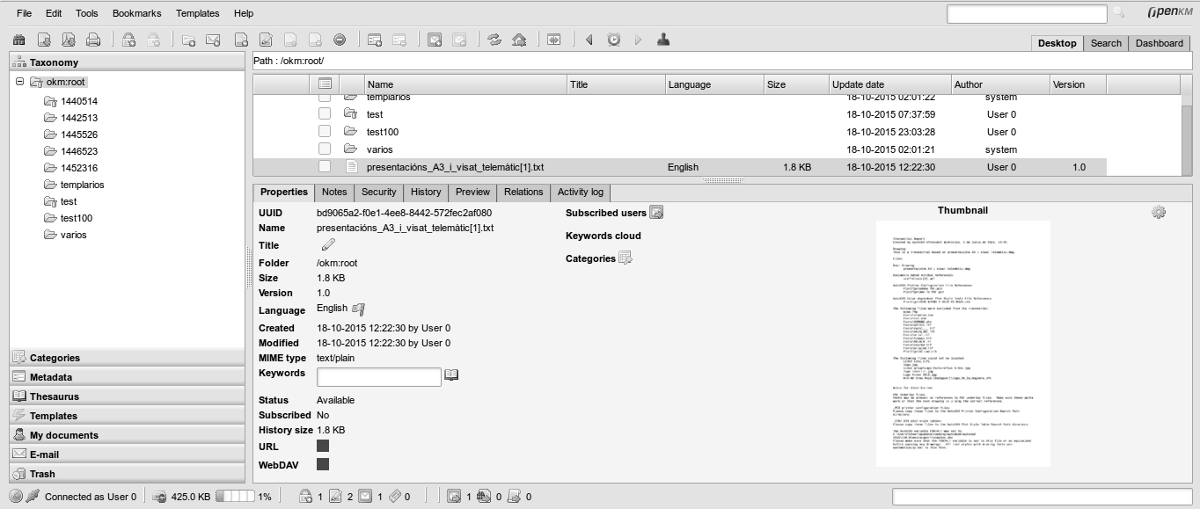
\includegraphics[width=\textwidth]{Masterarbeit_Bilder/openkm.png}
    \caption{Startseite der Webanwendung OpenKM}
    \label{openkm:home}
\end{figure}  


Das hier erstellte System nutzt einen anderen Ansatz zur Datenbeschaffung und Datensuche. Diese Suche beschränkt sich im Rahmen dieser Arbeit auf einfache Mustervergleiche und erlaubt das Suchen von Dateien über mehrere Peers hinweg anhand ihrer gesammelten Meta-Informationen. 




\chapter{Technische Analyse}
\label{chap:techAnal}
\chapmd{ Eine Weisheit der Dakota-Indianer}{,,Wenn Du entdeckst, dass Du ein totes Pferd reitest, steig ab.''}
 
Auffällig ist, dass die meisten Systeme in Java programmiert sind, wenn es um große Dateien geht, die auch noch plattformübergreifend angeboten werden. Die Schwächen des HTTP kommen gerade bei großen Dateien zutage und die dadurch aufkommenden Probleme bleiben ungelöst. Das zeigt sich in der Nutzung von WebDAV sowie bei Downloads \cite{davlimit}, \cite{httplimit}.

Es muss das richtige Protokoll für den jeweiligen Anwendungszweck verwendet werden.

\section{Warum Java}
Die plattformunabhängigen Anwendungen nutzen naheliegenderweise Java als Programmiersprache. Auch Scriptsprachen verwenden neben passendem Interpreter, meist in C/C++, die Java Plattform. Bekannteste Vertreter sind Python und Ruby.
Seit Java Version 7 ist die Einschätzung von James Gosling ,,Java ist wie C++ ohne Pistolen, Messer und Clubs." technisch nicht mehr haltbar, da mit Einführung von Java 8 und den Funktionalitäten, wie z. B.  \href{http://www.oracle.com/technetwork/articles/java/trywithresources-401775.html}{automatic resource management} und \href{http://www.oracle.com/technetwork/articles/java/rich-client-lambdas-2227138.html}{Lambda}, die Möglichkeit geschaffen wurde, andere Programmierkonzepte in der Sprache zu verwenden.

Auch für die Programmierung von Weboberflächen bietet Java mit \href{http://www.oracle.com/technetwork/articles/java/enterprise-html5-2227136.html}{JSF und HTML} eine schnelle und einfache Möglichkeit, Web-Anwendungen zu erstellen.

Die riesige Entwicklergemeinde hat auch viele Bibliotheken hervorgebracht, deren Ergebnisse heute in anderen Sprachen zur Anwendungsrealisierung verwendet werden. Die bekanntesten von ihnen werden von der
\href{http://www.apache.org/}{ Apache Software Foundation } gepflegt.


%% stolpern hier ....
Was Windows dieses Jahr mit {.NET} startete, hat Java lange zuvor durchgeführt. Durch die gemeinsame Open-Source Basis und der Möglichkeit die Virtuelle-Maschine legal mit in sein Programm zu integrieren erlaubt eine sehr einfache Anwendungsbereitstellung und Erstellung eingebetteter Anwendungen. Nachfolgend bezieht sich die technische Analyse auf die Realisierbarkeit in einer Java Anwendung.


\subsection{Arbeiten mit Dateien}
Bei der Realisierung gibt es trotz plattformunabhängiger API Schwierigkeiten. Ursachen sind Verhaltensunterschiede im Betriebssystem.
Es gibt allerdings einige grundlegende Informationen, wie dem Dateinamen, Dateipfad, Größe oder letzte Änderung, die sich mit leichten Abweichungen auf allen Plattformen finden lassen.

Bei der Verschlagwortung handelt es sich um ein Anhängen von Informationen. Diese Informationen sind bei der Speicherung nicht nur plattformabhängig, sondern unterscheiden sich bereits erheblich innerhalb des verwendeten Dateisystems einer Plattform.
Die meisten Betriebssysteme nutzen dabei erweiterte Attribute. Inwieweit bei Mac OS und Windows \acrshort{ads} oder \acrshort{rf} Verwendung findet, wurde nicht geprüft.  
 
Die einfach klingende Idee, Rechenzeit zu sparen, indem man Informationen voranalysiert und an die Datei anhängt, kann jedoch schnell durch einen Anwender oder ,,falsch'' funktionierendes Programm zunichte gemacht werden. Am Beispiel von Prüfsummen zeigen sich die Probleme bereits lokal auf dem Computer. Dazu berechnet ein Programm zu einer gegebenen Datei eine Prüfsumme und hängt das Ergebnis der Berechnung an die Datei an. Hier muss davon ausgegangen werden, dass das Dateisystem ebenso wie das Betriebssystem alle nötigen Funktionen bietet.

\bigskip
Dann können folgende Ereignisse eintreten:
\begin{itemize}
	\item Änderungen an der Datei sorgen für eine nicht mehr gültige Prüfsumme in den Attributen.\\
    Lösung: Zeitstempel der Prüfsumme mit anhängen und neu berechnen bei Abweichungen des Prüfungszeitpunktes zum Modifikationsdatum.
    
	\item Update verpasst. \\
     Lösung: Sollte der Verdacht existieren, dass sich die Datei geändert hat und dies, ohne Änderung im Änderungsdatum, sollte eine neue Berechnung erzwingbar sein.
     Auslöser könnten Programme sein, die neben dem Inhalt der Datei auch deren Meta-Informationen verändern. Wie mit diesem Problem umgegangen werden sollte, wird, da nach Aufgabenstellung eine Berücksichtigung solcher Programme nicht erfolgen sollte, nicht weiter beachtet.
\end{itemize}

Geht man davon aus, dass die verwendeten Programme Dateien nur mit ,,echten'' Änderungen neu schreiben oder erweitern, so ist es naheliegend, einen zweiten Prozess zu entwickeln, der die berechneten Informationen verarbeitet.

Es gibt zwei mögliche Ansätze zur Realisierung: {Polling} oder {Interrupt}. Nachteile beim Polling sind unregelmäßiges Reagieren auf Änderungen und Erzeugung von zu viel CPU Last. Ein weiterer Nachteil ist, dass zu schnell hintereinander erfolgte Änderungen übersehen werden können.

Für das Nutzen von {Interrupts} muss das Betriebssystem passende Schnittstellen bereitstellen. Ein {Interrupt} wird anschließend für ein bestimmtes Ereignis, wie Erstellen oder Ändern einer Datei, angemeldet und vom Betriebssystem sowie von der passenden Hardware verwaltet. Im Fall der Dateiüberwachung wird von den meisten Betriebssystemen eine Ordnerüberwachung angeboten, die sich zum gewünschten Vorhaben, beispielsweise durch Filterung, anpassen lässt. Dieser Ansatz übersieht keine Änderungen und stellt auch keine unnötigen Nachfragen. Das Programm benötigt dadurch kaum CPU-Rechenzeit.


\section{Kommunikation}
Mit Java stehen eine Menge Bibliotheken zur Auswahl. Im Abschnitt (\ref{sec:comm}) wurden zwei der größten Vertreter zur Kommunikation genannt. Realisiert wurde die Anwendung unter \acrshort{jms}, anders als  \href{http://xmpp.org/extensions/xep-0060.html}{,,XMPP (draft) XEP60''} stellt dieses eine etablierte Kommunikationsschnittstelle bereit, in der eine nachrichtenbasierte verteilte Anwendung programmierbar ist.

Zwischen Anwendungsserver und Client wird HTTP verwendet, um HTML Dokumente auszuliefern. Die Implementierung erfolgt auf HTTP 1.1 Grundlage. Kommende Versionen wie Java 9 nutzen bereits das von Google vorangetriebene HTTP 2 \cite{httpx1}, \cite{httpx2}.

Die Clients selbst sprechen -- wie in  Abbildung \ref{fig:ist-struktur2} ausgeführt -- zwischen den jeweiligen Servern bereits ein geeignetes Protokoll für den Datentransfer. Daher ergibt sich in der Kommunikation eine heterogene Landschaft, die die Vorgabe erfüllt, skalierbar zu sein. Man geht davon aus, dass der Dateitransfer zwischen Server und Client durch das passende vom Betriebssystem empfohlene Protokoll skalierbar ist. Eine Skalierbarkeit des Anwendungsserver  steht außer Frage. Es wird auf weiterführende Literatur verwiesen, um den hier verwendeten Anwendungsserver beispielsweise im Cluster zu betreiben \cite{glassfishcluster}.
Die hier erstellte eingebettete Version unterstützt allerdings einen Cluster Betrieb nicht und erfordert für eine Lastverteilung mehr Konfiguration auf den einzelnen Peers. Nachteilig ist zudem die dadurch entstehende höhere CPU und RAM Last.
 
\section{Sicherheit}
Die Anwendung verwendet keine Verschlüsselung im eingebetteten Modus. Üblicherweise muss dazu ein ,,selbst signiertes Zertifikat'' erzeugt werden, welches i. d. R. nicht in Webbrowsern vertrauenswürdig ist und ein direktes Arbeiten mit der Anwendung verhindert. Ein vorheriges Verteilen des Zertifikates und dessen Installation sind notwendig für einen reibungslosen Betrieb. Die nötige Arbeit entsprechender Realisierung wurde in andere Aufgabenbereiche verlagert. Die grundlegenden Algorithmen werden bereits durch die Bibliothek der ,,Legion of the Bouncy Castle'' bereitgestellt \cite{javabc}.

Ein Ausführen der Webanwendung über einen Proxy mit \acrfull{tls}, Verschlüsselung ist jedoch einfach, daher ist es ratsam, diesen Dienst zu verwenden, um eine Verschlüsselung für die Anwendung zu nutzen.

Ebenso kann eine Nachricht, vom \acrshort{jms}, durch beispielsweise SSH Port-Weiterleitungen durch einen verschlüsselten Tunnel versendet werden. Diese Dienste sind weitgehend transparent über der Anwendung nutzbar.
Die Kommunikation mit einem E-Mail-Server erfolgt über Javas interne \acrshort{tls}  da hier ein ,,vollständiger'' Client implementiert ist. Die Anwendung akzeptiert hier alle Zertifikate und umgeht dadurch die Schutzmechanismen, da auf den Testsystemen keine ,,echten'' Zertifikate vorliegen.
Diese Prüfung kann mit entsprechender Konfiguration geändert werden, so dass nur noch konfigurierte Zertifikate erlaubt sind. Dazu muss das Java-Tool keytool verwendet werden, um dem Java System entsprechende Zertifikate mitzuteilen.

Sicherheitstechnisch zu bedenken bleibt es, dass ein Peer, welcher sich zu einem Server verbindet, diesem vollständig vertraut.
Selbst wenn die Kommunikation zwischen den Peers sicher gestaltet ist, kann die Anwendung durch Konfigurationsschwächen und Anforderungen wie der Befehlsausführung, der Vorfilterung von Daten durch externe Prozesse, über die  Weboberfläche erhebliche Sicherheitslöcher in die bestehende Netzwerklandschaft reißen.

Der abhörsichere Transport und die Sicherheit in der Kommunikation unter den Peers geht dabei weit über die eigentliche Aufgabe hinaus und muss getrennt betrachtet werden. Um sich für eine geeignete Sicherheit entscheiden zu können, muss das System jedoch erst getestet werden. Ein ,,public/private key'' Verfahren könnte dabei genauso wie das Erzeugen einer zentralen Zertifizierungsstelle in das erstellte System etabliert werden.

Bis zu einer entsprechenden Entscheidung sollte das System bei Bedarf durch TLS Proxy oder HTTPS aus einem anderem Webserver außerhalb des eingebetteten Modus  oder durch SSH mit Port-Weiterleitungen durch den Tunnel für die Clients betrieben werden.


 
%%  ----- NEW ----



\section{Anwendungsserver}
\label{chap:appserv}
Die Anwendung baut auf einigen etablierten Bibliotheken im Java Umfeld auf. Als Server im eingebetteten Modus wird ,,Glassfish'' verwendet.
Lösungen mit Tomcat oder Jetty konnten wegen der JSF-API nicht verwendet werden, da viele genutzte Funktionen nicht vorhanden sind und es mehr Aufwand bedeutet, diese zu integrieren. Es gibt neben der gängigen Literatur im Internet auch Bücher, die das Einrichten und die ersten Schritte beschreiben wie \cite{glassfishee7}. Da sich aber für das Einbetten in die Anwendung beim ,,master'' entschieden wurde, werden nötige Konfigurationen vom Programm selbst erledigt.
Die Entscheidung für einen eingebetteten Anwendungsserver ist darin begründet, dass die Administration möglichst einfach gehalten werden sollte.
Tests zwischen Linux und Windows benötigten einen großen Konfigurationsaufwand und sind für normale Anwender ohne Vorwissen und Grundlagen nicht möglich den Server zu konfigurieren.


\subsection{Webanwendungen}
Heutige moderne webbasierte Anwendungen im Java Umfeld werden mittels {JSF} erstellt. So kann sich ein Java-Entwickler auf Java fokussieren und muss sich nicht hauptsächlich mit den Anforderungen von HTML und Javascript auseinandersetzen, da viele notwendige Scripte und Elemente automatisch erzeugt werden. HTML5 stellt nicht alle Eingabeelemente wie vom Desktop bekannt bereit. Meist werden diese durch Implementierungen wie \href{http://primefaces.org/}{{primefaces}} ergänzt. Diese nutzen meist gängige {CSS} und {JavaScript} Bibliotheken wie \href{http://getbootstrap.com/}{Bootstrap} und \href{https://jquery.com/}{jQuery} für erweiterte Eingabeelemente und visuelle Effekte.

Mit JSF  werden vorzugsweise HTML-Seiten generiert und durch das { binding} Konzept wird das Entwickeln in Java vereinfacht.
Mit { bindings} lassen sich Objekteigenschaften an HTML-Elemente koppeln, so dass das Zurückspeichern der über HTTP übertragenen Daten nahezu automatisch erfolgt.

\subsection{Contexts and Dependency Injection}
%%--monstersatz
Bei \acrfull{cdi} werden Objekte verwaltet und dadurch die Möglichkeit geschaffen, Abhängigkeiten, die zur Laufzeit entstehen, im Betrieb einzufügen und erst anschließend die entsprechende Methode aufzurufen. Dadurch lassen sich viele Entwurfsmuster wie z. B. das Interceptor-Muster einfacher implementieren und es müssen nur die entsprechenden Notationen an die Methoden geschrieben werden \cite{schmidt2002pattern}, \cite{gamma2011entwurfsmuster}, \cite{bien2003j2ee}. Das Muster lässt sich für das Einbauen von transparenten Transaktionen oder Log-Meldungen verwenden. Nachteile sind die schwere Nachvollziehbarkeit der Programmabläufe, da nicht wirklich klar ist, was an einer bestimmten Stelle injiziert wird.

Es ist darauf zu achten, dass alle Objekte im sogenannten {CDI-Kontext}, vom CDI-Container, meist innerhalb des Anwendungsserver, verwaltet werden. Werden neue Objekte benötigt, muss mit entsprechenden Notationen dem Container dies mitgeteilt werden.

\bigskip
Die wichtigsten Muster sind:

\begin{itemize}
    \item Interceptor, \cite{schmidt2002pattern}
    \item Dekorator-Muster, \cite{gamma2011entwurfsmuster}
    \item Chain-of-Responsibility, \cite{gamma2011entwurfsmuster}
    \item Proxy-Muster, \cite{gamma2011entwurfsmuster}
    \item Data Access Object (DAO) Muster, \cite{bien2003j2ee}
\end{itemize}

Wird {CDI}, {JSF}, {JPA} in einer Anwendung verwendet, ergeben sich Synergien. So können Konfigurationen von Datenbanken lose gekoppelt werden und deren Transaktionen bei Bedarf durch einen Interceptor gestartet werden. Programme die, {CDI} und {JPA} einsetzen, verwenden meistens das ,,Data Access Object''-Muster, welches notwendige Funktionen zum Datenspeicher nochmals vor der speichernden Anwendung kapselt. Es wirkt dadurch als Fassade vor der Datenbank und stellt sicher, dass nicht jedes Objekt eine eigene Suche implementiert und damit doppelten Code erzeugt.

Die Kombination von {CDI} und {JSF} vereinfacht die Verwendung von ,,Java Beans'', indem in andere Objekte Eigenschaften injiziert werden können. Diese Flexibilität ist bei Webanwendungen und dessen Formulare sehr wünschenswert, da einerseits Browser-Weichen so indirekt durch Muster wie  ,,Chain-of-Responsibility'' dem richtigen HTML-Generator übergeben werden können und andererseits durch das ,,lifecycle management'' auch Session und Request Kontexte einfach verwendbar werden. 

Durch die Aktualität von Java 8 gibt es noch viele Probleme im Zusammenspiel mit nicht aktualisierten Bibliotheken. Es werden mit den neuen Streams beim Evaluieren falsche Referenzen verwendet, welche zu einer ,,Nullpointer Exception'' führen. Kontexte mit Javas ,,lambda'' Funktionen, sofern diese etwas komplexer sind, führen zu falschem Verhalten in der Anwendung.
An dieser Stelle muss von der Verwendung von Java 8 Konzepten teilweise abgesehen werden, bis die Implementierungen des Containers die neuen Sprachelemente vernünftig unterstützen.




\subsection{Java Persistence API}
\label{chap:jpa}

Das \acrfull{jpa} kann alternativ zu {JDBC} eingesetzt werden und dient in Java Anwendungen der Datenbankkommunikation. Das darin integrierte \acrfull{orm} erledigt die mühsame Arbeit, Tabelleninhalte in Objekte zu überführen. Durch Notationen an den Java-Klassen wird die XML basierte Konfiguration auf ein Minimum beschränkt und die ,,persistence.xml'' enthält teilweise nur noch die Verbindungsdaten zur Datenbank.

Vorteile der Notationen im Code gegenüber der alten {XML} basierten Konfiguration ist die Möglichkeit der Prüfung durch den Compiler. Javas integrierte Zyklenerkennung wird beim \acrshort{orm} verwendet, um bei komplexeren Datenstrukturen redundante Speicherung zu vermeiden \cite{inden2012weg}.


%% -- ralf?
Dabei gibt es verschiedene Ansätze, der effizienteste ist das Erweitern einer Klasse für direktes Arbeiten auf der Datenbank. Das wird durch die Bibliothek während des Compilierens oder zur Laufzeit erledigt. Vergleichbare  Lösungsansätze müssen sich der Reflection-API behelfen und Verfahren wie die Zyklenerkennung selbst entwerfen.
Optimierungspotential gibt es zudem durch angepasste SQL-Ausdrücke und der Nutzung von Datenbank spezifischer Funktionen genügend.

Die Problematik, dass in jedem Objekt die Datenbankinformationen ständig mit gespeichert werden, wird mittels {,,detach''} Operation vermieden. Leider verzichtet man dadurch auf die Objektverwaltung und Funktionen wie dem {lazy loading}, welche Daten erst bei Bedarf von der Datenbank liest, was in Anwendungen die große Datenmengen verarbeiten viel RAM spart und die Anwendung beschleunigt.

Im  Zusammenhang mit Java 8 sind auch bei \acrshort{jpa} Probleme zu finden. Hier muss wiederum bedingt durch die Bibliothek gänzlich auf Java 8 verzichtet werden.
Dies liegt an der internen Erweiterung von Java-Klassen. Mit \href{http://openjpa.apache.org/openjpa-2.4.x.html}{OpenJPA 2.4} wurde eine Java 8 Unterstützung implementiert. Leider ist der verwendete Anwendungsserver mit \href{http://www.eclipse.org/eclipselink/}{EclipseLink} ausgestattet und die neue Version erst am 30.9.2015 erschienen, so dass zum Planungszeitpunkt noch keine entsprechende Unterstützung existierte.




\chapter{SCISERVER}
\chapmd{ Johann Wolfgang von Goethe (Werk: Wilhelm Meisters Wanderjahre)}{,,Es ist nicht genug, zu wissen, man muss auch anwenden; es ist nicht genug, zu wollen, man muss auch tun.''}


In diesem Kapitel wird die Anwendungsrealisierung beschrieben. Vorweg wurde sich bei der Realisierung auf die wichtigsten Funktionen konzentriert, so dass Sicherheitsaspekte nicht explizit beachtet wurden. Es werden Verschlüsselungsverfahren lediglich zur Authentifizierung verwendet. Die Anwendung wurde in mehrere Projekte strukturiert und durch das Build-Tool \href{https://maven.apache.org/}{{Maven}}  lässt sich das Projekt in allen gängigen \acrshort{ide} entwickeln. 


\bigskip
Ein Rückblick auf die Zusammenfassung zeigt, wie welche Aufgaben von der Anwendung erfüllt werden:

\begin{itemize}
     \item Zuordnung einer Datei der entsprechenden Person als Besitzer/ Verantwortlicher sowie zu den diversen Konten an den entsprechenden Servern und Endgeräten. \\
    Die Dateibesitzer-Informationen werden aus den Dateien ausgelesen und durch die manuelle Benutzerverwaltung dem entsprechenden Anwender zugeordnet. Dazu wird eine Zuordnung zwischen Computeraccount und Anwendungsanwender hergestellt, wie in  Abbildung \ref{fig:app-cfg-datei} zu sehen ist.
    \begin{figure}[htbp] 
        \centering
        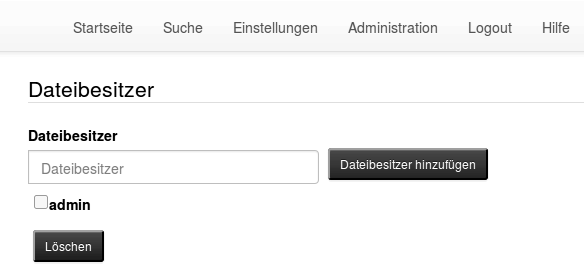
\includegraphics[width=0.9\textwidth]{Masterarbeit_Bilder/einstellungen_dateibesitzer.png}
        \caption{Dateibesitz einem Anwender zuordnen}
        \label{fig:app-cfg-datei}
    \end{figure}  
    
    
    \item Auslesen der Informationen einer Datei unter Beachtung des Dateisystems.\\
    Die Aufgabe wird durch die Java interne API erledigt, dabei wurde für die Attribute eine kleine Abstraktion erstellt, um diese in UTF-8 Kodierung zu schreiben bzw. lesen. 
    
       
    \item Anzeigenanpassung und individuelle Unterstützung je nach verwendeter Plattform.\\
    Es wird  der ,,User-Agent'' durch die Weboberfläche ausgelesen, um entsprechende Scripte für die verwendete Plattform zu liefern, wie in Abbildung \ref{fig:app-details} durch ,,open - dir'' oder ,,open - file'' ersichtlich ist.
    Die Anwendung nutzt native Anwendungen wie den Dateimanager zur gewohnter Benutzerunterstützung. Leider lassen sich wegen der Weboberfläche und den dadurch existierenden Sicherheitsbeschränkungen nur schwerlich  Anwendungen erstellen, in denen der Anwendungsbruch kaum spürbar ist. Für eine bessere visuelle Oberfläche wird auf den Endgeräten eine native Anwendung benötigt und keine Weboberfläche. Die Aufgabenstellung sah dies nicht vor. In der Anwendung ist die Integration daher nur durch Script-Downloads möglich. 
    Sollten die Informationen vom Client nicht richtig sein, wird dem Anwender eine Auswahl wie in Abbildung \ref{fig:app-details} gezeigt. Entsprechend der bekannten Plattformen wird ein Link generiert den der Anwender stattdessen verwenden kann.
    
        \begin{figure}[htbp] 
            \centering
            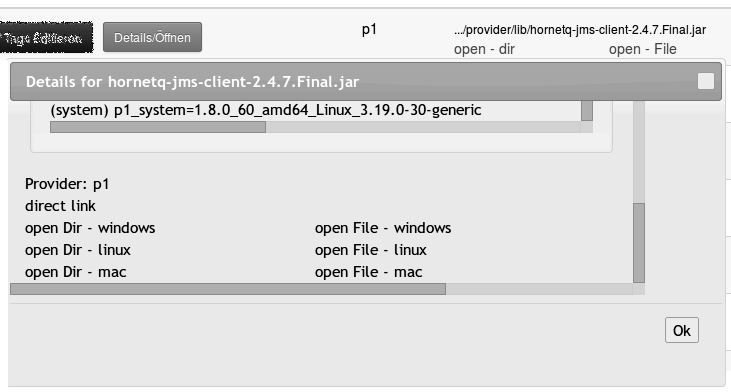
\includegraphics[width=0.8\textwidth]{Masterarbeit_Bilder/details_file.png}
            \caption{Integration in die Plattform, durch Scripte hinter Links}
            \label{fig:app-details}
        \end{figure}  
        
    
    %% ---ralf?
    \item Übertragung der Dateien zwischen teilnehmenden Computern\\
    Diese Aufgabe konnte leider nicht vollständig erledigt werden, der Mediator vermittelt zwar zwischen den einzelnen Peers, diese stellen aber ihre Funktionalität nicht durch eine geeignete Benutzeroberfläche zur Verfügung.
    
    \item Benachrichtigung über den Vorgang, wie Kopieren, Erstellen und Löschen einer Datei\\
     Dateien ohne Schlagworte werden periodisch Benachrichtigungen dem entsprechenden Anwender gesendet. 
     Mit minimalen Anpassungen können auch Hinweise zum Kopieren oder Erstellen erfolgen.
     Auch in der Weboberfläche sind diese Dateien sichtbar, sowie auf der Startseite Abbildung \ref{fig:app-ohnetags}, sofern der Anwender auch Dateibesitzer ist.
     
     \begin{figure}[htbp] 
         \centering
         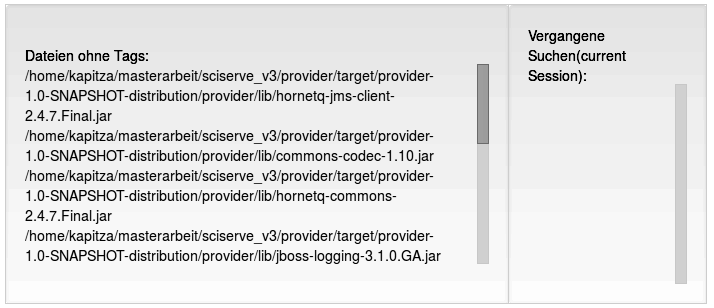
\includegraphics[width=0.8\textwidth]{Masterarbeit_Bilder/ohnetags.png}
         \caption{Dateien ohne Schlagworte}
         \label{fig:app-ohnetags}
        \end{figure}  
        
         
      \item Persistente Speicherung aller Informationen zu einer Datei, über die vom Dateisystem unterstützten Funktionen hinaus\\
      Die Informationen werden in einer eingebetteten Datenbank durch einen Peer gespeichert.
    \item Verlinken der \acrshort{dms}\\
    Durch eine ,,bridge'' ist es den Anwendungen möglich, Informationen unter einander auszutauschen. 
    \item Erkennung doppelter Dateien\\
    Hier ist keine explizite Anzeige erstellt. Doppelte Dateien können hier über einen ,,Workaround'' gefunden werden, indem die Prüfsumme in der Suchmaske eingegeben wird. Diese ist für jede Datei eindeutig, sollte die Datei also doppelt existieren, wird das Ergebnis alle Dateien auflisten. Wie Abbildung \ref{fig:app-dups} zeigt, ist hier die Datei ,,provider-1.0-SNAPSHOT.jar'' auch in einem Unterordner ,,lib'' doppelt vorhanden. Die Prüfsumme wird dabei durch ein ,,\%'' abgekürzt. Auf die Eindeutigkeit ist dabei jedoch selbst zu achten. 
    
    \begin{figure}[htbp] 
        \centering
        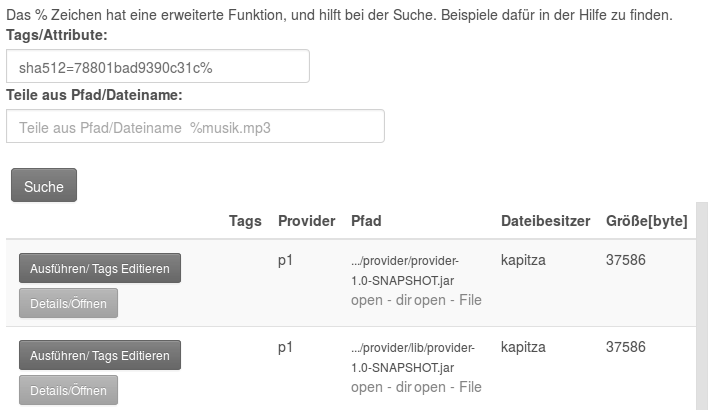
\includegraphics[width=0.9\textwidth]{Masterarbeit_Bilder/suchedups.png}
        \caption{Doppelte Dateien finden durch Prüfsummensuche}
        \label{fig:app-dups}
    \end{figure}  
    
    
    
\end{itemize}



\section{Dateiübertragung}
Dateiverbindungen finden im \acrshort{p2p} direkt zwischen den Peers statt.
Das kann bei IPv4 wegen \acrshort{nat} jedoch schnell zu Problemen führen. Der Fall, dass die Peers untereinander nicht die gleichen Protokolle sprechen, ist jedoch selten. Kritisch bleibt je nach Firewall-Typ ein Verbindungsaufbau. In der Abschlussbetrachtung wird auf einige Probleme der Datenübertragung noch einmal gesondert eingegangen, speziell welche Schwierigkeiten sich im Rahmen der Realisierung ergeben haben.

Das Protokoll sieht bereits entsprechende Befehle zum Datenaustausch vor. Diese werden jedoch nicht in der Weboberfläche einfach nutzbar angezeigt. Durch das Veröffentlichen einer Datei wird im System zwar deren Synchronisieren angestoßen, jedoch ist das Steuern der Empfängerpeers nicht möglich.

Durch die Freigabe des Befehls an dem entsprechenden Peer wird dieser angewiesen seine Daten freizugeben. Ob und wann das Empfangen fertig ist, lässt sich im aktuellen Protokoll jedoch nicht verfolgen. 

\bigskip
Schematisch lässt sich der Ablauf wie folgt beschreiben:

\begin{itemize}
\item Peer A erhält den ,,publish''-Befehl für eine Datei von einem Anwender
\item Peer A sendet Meta-Informationen über die Datei zu allen verbundenen Peers.
\item Jeder Peer prüft bei sich, ob er die Datei besitzt.
\\ Wenn: \\
-- Ja: Kopiert er diese zum angefragten Ziel, sollte diese dort nicht vorhanden sein.\\
-- Nein: Nachfrage beim anbietenden Peer erzeugen.
\item Jeder nachfragende Peer öffnet einen Port und ermittelt seine externen Verbindungsparameter.
\item Die Verbindungsparameter werden mit Dateiwunsch an alle verbundenen Peers gesendet.
\item Die Peers, welche die Datei besitzen, senden die Informationen zum Nachfragenden.\\
Der Dateitransfer findet direkt zwischen den Peers statt und stört keine weiteren Teilnehmer.
\end{itemize}

In Anlehnung an die in Kapitel \ref{sec:ist} erläuterten Prämissen soll sich die Anwendung einfach in das bestehende Netzwerksystem integrieren. Dazu werden weitere Dienste auf dem Server (vgl. Abbildung \ref{fig:xist-server}) benötigt.
 
Die Endgeräte sind von der Anwendung nicht betroffen. Diese arbeiten wie gewohnt mit ihren Netzwerklaufwerken weiter.
 
\bigskip
 
 \begin{figure}[htbp] 
     \centering 
     \begin{tabular}{|p{.45\textwidth}|}
         \hline
         Server\\ \hline\hline
         ein oder mehrere Dienste wie:\\
         master  | database | provider | www | bridge\\ \hline\hline
         NFS | SMB| Appeltalk | \ldots \\ \hline
         Betriebssystem \\ \hline
         Netzwerk (TCP /IP) \\ \hline
        \end{tabular}
        
        \caption{Server}
        \label{fig:xist-server}
        
    \end{figure}   
    
 
Da es sich um eine \acrshort{p2p}-Lösung handelt, müssen nicht alle Dienste auf jedem Server laufen. 
Teile der Anwendung werden von bestimmten Peers bereitgestellt und ergänzen sich zu einer Anwendung, die durch eine Weboberfläche bereitgestellt wird.


In Anlehnung an die ersten \acrshort{p2p}-Netzwerke wie z. B. Napster stellt das ,,master''-Projekt den Kern des Netzwerkes \cite{mahlmann2007peer}.
Dabei kann eine komplexe Konfiguration wie in Abbildung \ref{fig:app-outline} aussehen. Es ist natürlich auch möglich alle Peers auf einem Computer oder in virtuellen Maschinen zu installieren.

\begin{figure}[htbp] 
    \centering
    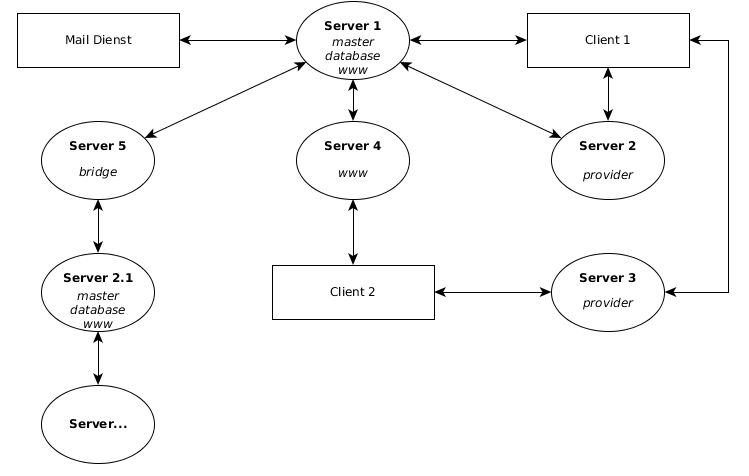
\includegraphics[width=0.8\textwidth]{Masterarbeit_Bilder/clients_uebersicht.png}
    \caption{Übersicht und mögliche komplexere Konfiguration}
    \label{fig:app-outline}
\end{figure}  


 

Hier existieren, neben den diversen Server, zwei Clients. Die Clients können über die mit einem ,,provider'' versehenen Server Dateisuchanfragen an die ,,database'' stellen.
In der zentralen Datenbank werden die Dateiinformationen gespeichert, um Verschlagwortung und weitere Attribute zu unterstützen.
Ersichtlich ist, dass Lastverteilung durch Erzeugen weiterer Peers einfach zu realisieren ist. 

Datensicherung kann prinzipiell durch eine ,,bridge'' erfolgen. Diese ersetzt aber nicht die Möglichkeit einer im Cluster betriebenen Datenbank und ist damit auch nicht vergleichbar. Ein Umstellen der Datenbank erfordert lediglich kleine  Anpassungen  in der Konfiguration  der Anwendung ,,database'', um die gewünschten Verbindungsparameter bereitzustellen.


\section{Die Projekte}

%% ralf?
Das Build-Tool \href{https://maven.apache.org/}{,,Maven''} verwaltet in den einzelnen Projekten auch deren Abhängigkeiten. Die Abhängigkeiten untereinander sind jedoch 
in der verwendeten Konfiguration nicht konfiguriert. Dazu wurde ein kleines Script verwendet, da ein weiteres Verwalten eines ,,multi module project'' mehr Zeit bedarf als die Projekte in der richtigen Reihenfolge aufzurufen. 

Die Kommunikationsschicht wird durch das ,,client'' Projekt bereitgestellt.
Die resultierende Bibliothek muss zum Erstellen weiterer Projekte in das lokale Repository installiert werden.
Da der ,,master'' von der ,,database'' und dem ,,www'' Projekt im eingebetteten Modus abhängig ist, sollten diese wie auch der ,,client'' zuerst gebaut werden.
Da die Installation der anderen Projekte nicht falsch ist, genügt ein Tippen von ,,mvn clean install'' in den entsprechenden Projekten, um entsprechende ausführbare Anwendungen zu erzeugen.

Nachfolgend wird nun auf die einzelnen Komponenten eingegangen und Funktionen sowie Konfigurationen beschreiben.


\subsection{Bridge-Projekt}
Mit dem ,,bridge'' Projekt wird die Idee der Erweiterung des Netzwerkes verfolgt. Wie in Abbildung \ref{fig:app-outline} sichtbar, verbindet dieses Projekt zwei autonome Systeme und ermöglicht einen Informationsfluss über die Systemgrenzen hinweg. Ein schöner Nebeneffekt ist das Synchronisieren der Datenbank im laufenden Betrieb. Da aber auch mehrfache Antworten auf eine Frage kommen können, müssen die Peers mit Duplikaten und leichten Variationen in den Antworten umgehen können.

Bei zu komplexer Konfiguration kann ein Peer auch mehreren Netzwerken angehören.
Dabei werden die Daten in beide Richtungen der ,,bridge'' gesendet. Diese Dopplungen können durch einen \acrfull{ttl} Wert nicht verhindert werden. Was aber ein \acrshort{ttl} vermeidet sind ,,round trips'' innerhalb des Routing.

Die Konfiguration ist einfach gehalten, sie erwartet die ,,master'' IP bzw. \acrfull{fqdn} Adressen sowie ein gemeinsames Geheimnis, um am entsprechendem Netzwerk teilzunehmen.

\bigskip
Beispielsweise lässt sich mit den acht nachfolgenden Zeilen in der ,,bridge.properties'' eine Verbindung zwischen zwei Systemen herstellen.

\begin{verbatim}
# Eindeutige ID der Bridge in beiden Systemen
de.bluepair.jms.client.id=bridge_host0_host1
de.bluepair.jms.autoconnect=true

de.bluepair.jms.masterkey.0=key1
de.bluepair.jms.ttl.0=1
de.bluepair.jms.host.0=ip1

de.bluepair.jms.masterkey.1=key2
...
\end{verbatim}


\subsection{Provider-Projekt}
Der ,,provider'' stellt Dateiinformationen und auch Dateien zur Verfügung. Er reagiert auf Anfragen des ,,master'', zu dem er eine Verbindung aufbaut hat, und ermöglicht einem Anwender des ,,www''-Peers eine konfigurierte Befehlsausführung. Sicherheitstechnische Aspekte müssen zu einem späteren Zeitpunkt geklärt werden. 

Gedacht ist die Kommunikation in erster Linie nur vom ,,provider'' in Richtung ,,master''. 
Wünsche, welche die Kommunikation unter den Peers beinhalteten, ergaben im Zuge der Entwicklung, dass die Prozessverwaltung in Java ähnliche Probleme wie die Dateiüberwachung aufweist. Diese Wünsche beinhalteten die Befehlsausführung mit externen Programmen aus der Weboberfläche. Viele wünschenswerte Informationen fehlen jedoch in den API und konnten dadurch weder am Prozess noch in der Weboberfläche abgebildet werden. Auf einfache Weise ist es in Java nicht möglich, Prozesse und deren ID oder OWNER herauszufinden.
Auch das Feedback von einem Prozess ist schwerlich zu überwachen, bei lang andauernden Hintergrundaufgaben wird in der Anwendung daher der Status nicht übermittelt. Es wird wohl auch hier nötig sein, eine weitere Fassade über das von Java bereitgestellte Prozessverwaltungssystem zu entwickeln.

Es kann zwischen internen und externen Befehlen unterschieden werden.
Interne Befehle wie ,,publish'' erlauben dem Anwender Dateien freizugeben, externe Befehle eigenen sich mehr für die Vorverarbeitung wie dem Extrahieren bestimmter Informationen.

\bigskip
In der Konfigurationsdatei ,,provider.properties'' können Befehle einfach angemeldet werden.

\begin{itemize}
    \item Den internen Befehl ,,publish'' kann für die ,,www''-Anwendung freigegeben werden.
    Andere werden derzeit nicht unterstützt.\\
    \verb|publish.internal=true|
    
    \item Der externe Systembefehl ,,cat'' unter Linux wird durch zwei Einträge freigegeben. Einmal muss der Befehl als solcher definiert werden während deren Argumente, die meist anderen Regeln folgen, in der ,,www''-Anwendung mit Platzhaltern vorbelegt werden. Hier ist der Platzhalter ,,\{\}'' konfiguriert. Da  diese Sonderzeichen in Java eine spezielle Bedeutung haben, müssen die Zeichen geeignet maskiert werden.
    \\
    \verb|cat.path=/bin/cat|\\
    \verb|cat.replacewithpath=\\{\\}|
    
\end{itemize}

 

In der Konfigurationsdatei finden sich auch weitere optionale Parameter. Neben den Standardparametern wie \acrshort{fqdn} bzw. IP sind auch folgende Werte erlaubt:\\

\begin{itemize}
    \item Zeit in Millisekunden die vom Watchservice gewartet werden, bevor ein Event stattfindet. Hier wird der Wert auf ein Sekunde gesetzt.\\ \verb|de.bluepair.watchservice.polling=1000|

\item In Linux können Duplikate in den Events durch Angeben von dem Wert ,,true'' verhindert werden. \\
\verb|de.bluepair.watchservice.nodupes=false|

\item Das Programm benötigt Schreibrechte auf den Dateien, auf denen es die  Prüfsumme berechnet. Mit ,,true'' wird ein ständiges Neuberechnen erzwungen, was nicht zu empfehlen ist.\\
\verb|de.bluepair.watchservice.readonly.force=false|

\item Einige Befehle haben eine erzwingende Option.
Mit ,,true'' kann diese Verhalten dauerhaft abgestellt werden.
Damit kann ein Überschreiben von Dateien verhindert werden. Diese Angabe hat bei der Nutzung von externen Befehlen und Vorverarbeitungen  keinen Effekt.\\
\verb|de.bluepair.nodelete=true|

\item Wird kein port für den Dateitransfer angegeben, wählt die Anwendung durch das Betriebssystem einen beliebigen freien Port. Das Konfigurieren einer Firewall ist ohne konkreten Port schwer. Für Windows ist empfohlen einen Port festzulegen.\\
\verb|de.bluepair.provider.fileget.port=6666|
\end{itemize}

\subsection{Client-Projektbibliothek}

Das ,,client'' Projekt ist eine Bibliothek, die von Peers verwendet wird, um eine einheitliche Kommunikation zu gewährleisten. Es stellt eine API bereit, um einfach mit \acrshort{jms} zu agieren.

Es stellt zudem die oben erwähnte Abstraktion des Watchservice zur Verfügung, auf dessen Realisierung hier eingegangen wird. Das erlaubt Peers ein gezielteres Arbeiten mit Dateievents.

Zu den in jeder ,,PROJEKT.properties'' anzutreffenden Konfigurationen gehören:

\begin{itemize}
    \item
    Diese Einstellung lässt im Fehlerfall des Peers einen erneuten Verbindungsaufbau stattfinden.\\
    \verb|de.bluepair.jms.autoconnect=true|
    
    \item Die Kommunikation unter den Peers ist durch ein gemeinsames Geheimnis gesichert. Dieses wird i.d.R. vom ,,master'' festgelegt. Peers, die nur mit dem ,,master'' reden wollen, brauchen dieses in einfachsten Fällen nicht kennen. Das Geheimnis stellt bei einigen Befehlen sicher, dass hier keine unerwünschte Nachricht ausgeführt wird.\\  
    \verb|de.bluepair.jms.masterkey=sharedKey|
    
    \item Die Verbindung erfolgt über diesen Eintrag zu einem ,,master''-Peer.
    Dieser Peer stellt \acrshort{jms} und \acrshort{stun} für evtl. weitere andere Direktverbindungen bereit. Es wird kein vollständiger \acrshort{stun}-Dienst abgebildet, lediglich die IP- und Port-Adresse zurückgeschrieben\\
    \verb|de.bluepair.jms.host=IP_OR_FQDN|
    \item Jeder Client sollte im Netzwerk einen eindeutigen Namen haben. Es ist hier nicht notwendigerweise ein \acrshort{fqdn} nötig, jedoch bei großen Netzen zu empfehlen. Dieser Eintrag wird z. B. bei ,,www'' verwendet, um weitere Konfigurationen eines ,,provider'' einzustellen.\\
  \verb|de.bluepair.jms.client.id=UNIQUE_ID|
\end{itemize}


\subsubsection{Java NIO}
Das Java ,,new/non-blocking Input Output'' API ermöglicht Java Anwendungen seit Version 7 einen ,,WatchService'' zu verwenden. Dieser Service kann zur Ordnerüberwachung eingesetzt werden. Dabei werden ,,polling'' und ,,interrupt'' Ansätze unterstützt.

Leider wird von diesem Service bei einer Dateiänderung nur der Dateipfad zur Datei, nicht aber Auskunft über den Prozess, übertragen. Auch bei den Events mangelt es an fehlender Abstraktion. Nur mit CREATE, DELETE, MODIFY ist ein Arbeiten mit wissenschaftlichen Daten nicht sinnvoll. Ein ständiges Überprüfen, ob es sich um ein noch aktives Kopieren handelt, ist Ressourcen verschwendend. Eine neue Datei wird, wenn sie durch einer längeren Kopieraktion entsteht, mehrmals das Event MODIFY durchlaufen. Ein Event ONCOPY wäre für die Verarbeitung einer solchen Datei einfach zu verwenden und könnte durch ein FINISH als beendet markiert werden. So lassen sich ständige unnötige Neuberechnungen auf Dateiinhalte vermeiden.

Eine Fassade  über dem ,,WatchService'' sieht daher mehr als die in  ,,StandardWatchEventKinds'' bestehenden Events vor \cite{gamma2011entwurfsmuster}. So werden Events von der Fassade aggregiert und nur etwa alle 5 Sekunden weitergegeben. Eine abweichende Zeit lässt sich beispielsweise im ,,provider'' einstellen. Dabei werden bei Events auf dem gleichen Dateipfad folgende Regeln beachtet.

\begin{itemize}
    \item Auftreten von zwei MODIYFY Events \\
    löst ein ONCOPY und ein MODIFY Event aus.
    \item Auftreten von zwei ONCOPY Events\\
    löst nur ein ONCOPY Event aus.
    \item Auftreten vom letzten MODIFY Event nach Starten des ONCOPY\\
    löst ein FINISH Event im nächsten Zyklus aus.
\end{itemize}

Dadurch wird das Verwenden flexibler und das Unterdrücken von einigen Events wird vergleichbar wie beim Arbeiten mit Exception durch ,,addSuppressed'' und ,,getSuppressed'' noch nachvollziehbar gestaltet. Bei Bedarf kann so eine genauere Aussage zum Event gemacht werden.

%% --ralf?
Die Fassade kann der Problematik, den Änderungsprozesses zu erkennen, nicht zuverlässig entgegen kommen und liefert die Informationen daher auch nicht mit. Das Auslesen von Betriebssystemprozessen ist leider nicht trivial lösbar. Dieses Problem betrifft die Anwendung gleich zwei Mal.

Anders als der ,,WatchService'' gibt die Fassade den absoluten Pfad weiter, da sich damit einfacher arbeiten lässt als mit einer relativen Angabe zu einem zum Triggerzeitpunkt unbekannten Ordner.

Auch das Arbeiten mit erweiterte Attributen konnte so vereinfacht werden.
Durch ein entsprechendes Event werden alle nötigen Operationen, um Attribute lesen oder schreiben zu können, bereits vom Event bereitgestellt. Das Arbeiten mit diesem Event entspricht daher einer Fusion verschiedener einfachen Java-API wie ,,WatchEvent'', ,,Path'', ,,Files'' und ,,File''.

Es ergeben sich auch Nachteile bei der Verwendung  der Fassade. Events sind nicht mehr in Echtzeit übertragbar, da eine Verzögerung vor der Weitergabe entsteht. Dies steht aber mit den hier genannten Daten in keinem Konflikt. Es könnte jedoch passieren, dass Events veralten und ein Weiterarbeiten nicht mehr nötig oder möglich ist. Beispielsweise ist ein Kopiervorgang mit anschließendem direktem Löschen ein möglicher Kandidat für Fehler und muss bei Verwendung beachtet werden. Dabei könnte es passieren, dass ein MODIFY Event weitergegeben wird, welches keiner Datei mehr zugrunde liegt.
Um der Problematik ein wenig entgegenzuwirken, werden Events vor der Weitergabe geprüft, ob diese zum Prüfungszeitpunkt mit keinen bekannten Events in Konflikt stehen.

\bigskip
Dabei treten speziell die Konflikte auf:

\begin{itemize}
    \item MODIFY zu DELETE \\
    Wie oben erwähnt, kann eine Dateiänderung mit anschließendem Löschen die Änderung gänzlich eliminieren, da die Änderungen nicht mit übertragen werden.
    \item CREATE zu DELETE \\
    wegen Transitivität (CREATE -> MODIFY -> DELETE) verhält sich dieser Fall wie oben beschrieben.
\end{itemize}

Da es sich bei der Verwendung um einen Dienst zum Berechnen von Prüfsummen handelt, muss nicht zwangsweise sichergestellt werden, dass jede Änderung berücksichtigt wird und daher Änderungskonflikte durch ersetzendes Kopieren von Dateien nicht betrachtet werden.

Die Fassade selbst realisiert ein Beobachter-Muster, um ihre Dienste nach außen hin anzubieten \cite{gamma2011entwurfsmuster}.
Als Kommunikationsextra ist es möglich, der Fassade Events zu injizieren. So muss nicht zwangsweise eine Änderung auf dem Dateisystem stattfinden.

Diese Möglichkeit wird mit einem UPDATE Event realisiert.
Dabei steht dieses in Konflikt mit allen anderen Events. Es soll lediglich sicherstellen, dass auf jeden Fall mindestens ein Event im nächsten Ausgabetakt stattfindet.

Um Extra-Informationen an ein Event anzuhängen, wurden Events, wie bei den meisten Controls von JavaFX, mit den Methoden ,,getUserData'' und ,,setUserData'' erweitert. Dadurch lassen sich beliebige Objekte durch die Anwendung transportieren. 



\subsubsection{Java Mail}
Die Java Mail API wurde verwendet, um einen schnelleren Zugriff auf E-Mails zu bekommen. Dabei wurde die API so implementiert, dass diese mit den Funktionen aus Java 8 verwendet werden kann.

Eingehende E-Mails sind in dieser API nicht mehr vom Mail-Server getrennt und können direkt Antworten generieren und versenden. Das vermeidet unnötig viele Referenzen auf Objekte und erlaubt bei Verwendung ein einfacheres Arbeiten.

Die API muss, für die meisten Server, im Internet seit April 2014 Verschlüsselung verwenden \cite{sslmail}. Daher sind für die API weitere Konfigurationsparameter erforderlich.
\label{javamailc}
\begin{itemize}
    \item Zu den Standardparametern gehören die Verbindungsparameter zum Server.\\
    \verb|de.bluepair.mail.port=SMTP_PORT|\\
    \verb|de.bluepair.mail.host=IP_OR_FQDN|\\
    \verb|de.bluepair.mail.user=USER|\\ \verb|de.bluepair.mail.password=USER_PASSWORD| - das Passwort ist leider in Klartext anzugeben und wird für IMAP und SMTP verwendet. \\
    \verb|de.bluepair.mail.address=USER@FQDN| - die Sender-Adresse unter der E-Mails versendet werden. 
    \item Aus der Java Mail API können beliebige Parameter  durch Verwendung eines PREFIX \verb|de.bluepair.| aufgenommen werden.
    \verb|de.bluepair.mail.smtp.ssl.trust=*| und\\
    \verb|de.bluepair.mail.imap.ssl.trust=*| werden Standardmäßig gesetzt.
    
\end{itemize}

Wegen der verwendeten Testumgebung und der oben genannten Problematik, dass eine Verschlüsselung zwingend nötig ist, wurden die \verb|ssl.trust| Parameter Standardmäßig auf \verb|*| gesetzt. Dies hebelt einige Schutzfunktionen von Zertifikaten aus, es ist ratsam sich passende Parameter zu überlegen. Gegebenenfalls muss eine ,,socketFactory'' selbst erstellt werden. 

\subsection{Database-Projekt}

Der Kern für Suchen und Benachrichtigungen wird von dem ,,database'' Projekt bereitgestellt.
Das betrifft auch die Verwaltung der zusätzlichen Informationen einer Datei, die in einer SQL-Datenbank gespeichert werden. 
Die Anwendung kann mit eingebetteten Datenbanken oder extern wie z. B. {MySQL} oder {PostgreSQL} betrieben werden.
Durch \acrshort{jpa} ist innerhalb der Anwendung keine Anpassung nötig, da dieses SQL-Anfragen entsprechend dem Treiber der Datenbank erzeugt.

Durch den Anwendungsserver ist eine Konfiguration wegen der Zentralisierung sehr einfach gehalten, da hier alle benötigten Angaben zentral für alle auf ihm laufenden Anwendungen getätigt werden können. Es lassen sich diese Optionen auch durch einen \acrfull{acc} in einem Peer nutzen, jedoch ist die Bibliotheksauswahl durch Konflikte in Versionen schwerlich zu beheben. Zudem existiert die Problematik, dass im eingebetteten Modus nicht alle Konfigurationen zu Verfügung gestellt werden, so dass \acrshort{acc} keinen Mehrwert für die Anwendung bietet, da die Funktionen bereits auf Serverseite nicht zu Verfügung gestellt wurden.

Bei der Auswahl einer Datenbank muss lediglich darauf geachtet werden, dass diese auch unter Java lauffähig ist. 
Die Verwendung von \acrshort{jpa} ist zwar langsamer als das Schreiben von entsprechenden SQL-Anweisungen, der Vorteil liegt aber in der konsequenten Vermeidung von SQL-Injektion und direkten Nutzen von Objekten.


Alle Nachrichten, die am ,,master'' eingehen, werden von diesem an die Datenbank weitergeleitet und verarbeitet. Dadurch kann neben der reinen Speicherung auch eine Statistik erhoben werden. Das Benachrichtigungssystem, welches in diesem Peer realisiert wurde, versendet Erinnerungen anhand des Datenbestandes und versucht mit diesen den Anwender zu ermuntern, den Datenbestand zu verbessern.
Die dazu erzeugte E-Mail wird jedem registrierten Anwender durch die hinterlegte E-Mail-Adresse gesendet.

Das System beachtet dabei, ob überhaupt ein Anwender E-Mails empfangen will durch die Option \verb|email.push=true|, und versucht dabei die Adresse aus dem Login oder entsprechender Option \verb|email=MAIL@FQDN| zu erkennen.

Um die Häufigkeit der Benachrichtigungen zu steuern, kann in der Konfiguration neben den oben genannten Java Mail (\ref{javamailc}) Einstellungen die Zeitintervalle zum Versenden und Bearbeiten von E-Mails eingestellt werden.

\begin{itemize}
    \item Die Überwachung eines IMAP-Ordner muss dazu angegeben werden.\\
    \verb|de.bluepair.mail.mailbox=INBOX| - INBOX ist i.d.r. Standard
    \item Anschließend kann das E-Mail Verarbeitungsintervall wie unten auf z. B. 1 Sekunde eingestellt werden.\\
    \verb|de.bluepair.mail.imap.polling=1000|
    \item Das Erinnern via E-Mail kann unabhängig von der Verarbeitung festgelegt werden. Die hier erteilten 10 Sekunden sind nicht in der Produktion zu empfehlen, da dadurch gerade zur Einführungsphase eine erhebliche Menge an E-Mails versendet werden könnte.\\
    \verb|de.bluepair.mail.reminder=10000|
    \item Bei der Erzeugung von E-Mails wird ein Link für die Weboberfläche erzeugt. Um auch den richtigen Link zu erzeugen, wird der Port benötigt. Keine Angabe lässt den Port 8080 vermuten. Ein anderer wird durch \\
    \verb|de.bluepair.www.port=7070| angegeben. Als Host wird der Eintrag \\
    \verb|de.bluepair.www.host=FQDN| verwendet und bei keiner Angabe \\
     \verb|de.bluepair.jms.host=FQDN| der ,,master'' angenommen.
    
    \item Angaben für den einfachen \acrshort{stun} Dienst erfolgen mit \\
    \verb|de.bluepair.jms.echo.port=8888|
    
\end{itemize}
 
Dieser Peer nutzt zur Verarbeitung anders als alle bisherigen Peers eine Bibliothek für \acrshort{cdi} und Events. 
Das Verarbeiten von den eingehenden Nachrichten läuft dabei mehrstufig ab und nutzt ein Layer Architekturmuster \cite{buschmann1998pattern}.

Neue Dateien werden vor dem Speichern in die Datenbank auf ähnliche, bereits vorhandene Einträge untersucht.
Aktuell hilft dabei die Prüfsumme, so dass Tags, die von Anwendern vergeben wurden, auch direkt für neue Dateien gelten. Das vermeidet auch Erinnerungen für Duplikate und Sicherungen bestimmter Dateien zu versenden.

Handelt es sich um Datei fremde Nachrichten, wie Anfragen vom ,,www''-Peer, stellt die Anwendung eine einfache Benutzerverwaltung, die neben der üblichen Funktionen auch einem oder mehreren Anwendern Dateien zuordnen kann.

Die verwendete eingebettete Datenbank erzeugt sich komplett selbst, die Konfigurationen dieser können jedoch nicht ohne Änderungen am Code gemacht werden. Das Abstellen und Einrichten neuer Verbindungsparameter zu anderen Datenbanken erfordert daher grundlegende Programmiererfahrungen mit der \acrshort{jpa}.



\subsubsection{Mail Service}
Da bereits vorab auf die Konfiguration der E-Mail-Funktion eingegangen wurde, wird hier nur noch der Mehrwert für den Anwender beschrieben.

Die vom System versendete E-Mail ist so präpariert, dass ein Anwender durch Antworten auf diese E-Mail dem System die verlangten Informationen mitteilen kann.

Dazu darf der E-Mail-Inhalt nicht gelöscht werden, wichtig ist hier die Prüfsumme. Das System reagiert auf das Schlagwort \verb|TAGS=|, welches in der E-Mail verwendet werden soll, um Schlagworte der entsprechenden Datei zuzuordnen.



\subsection{Master-Projekt}

Der ,,master''-Peer stellt als eingebettete Version die größte  Funktionalität. Zu dieser gehört auch das Vermitteln der Nachrichten, um den Peers die Kommunikation zu ermöglichen. Wenn es darum geht, Dateien auszutauschen, finden sich einige Ansätze auch im FTP-Protokoll wieder \cite{rfc959}. 
Dazu zählen das Vermitteln der Ports, wie sie bei FTP in einer Server-zu-Server Kommunikation durch den Menschen (oder Script) erledigt werden.

Auch ein primitives \acrshort{stun} ist implementiert, um IP und Port eines Peers zu erkennen. Jedoch beschäftigt sich diese Arbeit nicht mit der Problematik des ,,Hole Punching'' und geht davon aus, dass Firewalls zwischen den Peers die Kommunikation erlauben.


Dieser Peer prüft die Kommunikation zwischen Peers, sofern diese untereinander reden wollen, auf den von ihm vergebenen gemeinsamen Schlüssel.
Die zwei Kommunikationskanäle unterscheiden sich in der Verlässlichkeit des Nachrichtentransports. Nachrichten an diesen Peer werden durch ein ,,Queue'' geregelt. Diese speichert die Nachrichten im Fall der Abwesenheit zwischen. Die Kommunikation zu allen anderen Peers sowie für diese untereinander wird durch eine ,,publish-subscrib'' Architektur geregelt. Sie erlaubt eine effiziente Kommunikation zu allen Peers, jedoch keine zuverlässige. Daher kann es sein, dass Nachrichten verloren gehen. Die Problematik wird durch Verwendung von TCP auf An- und Abwesenheit eingeschränkt. 

Die direkte Kommunikation zwischen den Peers beschränkt sich aktuell auf den Dateitransfer, da dessen Nachrichtenaustausch an ,,Napster'' angelehnt ist und immer über den Server läuft.


Im eingebetteten Modus werden alle nötigen Dienste gestartet. Dabei wird sich auf die nötigste Konfiguration beschränkt. Zu den eingebetteten Diensten gehören das \acrshort{jms}, ,,database'', ,,www'' und ein Anwendungsserver. Nachfolgend wird nur auf \acrshort{jms} und die speziellen Parameter für diesen Peer eingegangen, die weiteren können den entsprechenden Kapiteln entnommen werden.

\begin{itemize}
    
    \item 
    Ist dieser Parameter nicht angegeben, wird automatisch einer erzeugt. Er kann in der kleinen Shell durch den Befehl ,,masterkey'' oder der entsprechenden Konfigurationsdatei nachgesehen werden.\\
    \verb|de.bluepair.jms.masterkey=SHARED_KEY|
    \item Der Webserver kann auf einem beliebigen Port gestartet werden, damit kein Konflikt entsteht, wird per Standard \verb|7070| verwendet. Das kann in der Konfiguration mit \\
    \verb|jsf.port=7070| angegeben werden. \\
    Webanwendungen können durch den ,,deploy''-Befehl und Angabe von Datei, Name und Kontext als Parameter installiert werden, sowie durch ,,undeploy'' und Angabe des Namen zerstört werden.
    Für die Basisanwendung werden alle Kontexte überschrieben, es ist ein Neukonfigurieren nötig, um andere Anwendungen zu erlauben. Für die Basisanwendung wird automatisch der Befehl\\
    \begin{quote}
        deploy www.war www /
    \end{quote}
     abgesetzt.
     
     
     
     \item Die interne einfache \acrshort{stun}-Implementierung kann als Dienst durch \\
     \verb|ipecho.port=8888| auf einem beliebigen anderen Port verschoben werden. Andere angaben als der Standardport, müssen auch in den Clients angepasst werden.
     
     
    
\end{itemize}


Es gibt noch einige kleinere Befehle für die Shell, was das Debuggen vereinfachen kann. Dazu gehören ,,property KEY VALUE'', um eine neue Umgebungsvariable ,,KEY'' auf den Wert ,,VALUE'' zu setzen, und ,,send ...'', welches eine mit Leerzeichen getrennte Wortliste annimmt, um Nachrichten in das \acrshort{p2p}-Netzwerk zu senden. Der ..print'' Befehl lässt die Nachrichten auf der Konsole ausgeben.

Um wichtige Kommunikation wie das Vernetzen der ,,master'' und das Speichern getrennt zu halten, wurden weitere Kanäle  für die ,,bridge'' und ,,database'' eingeführt. Diese sind auch als eine ,,publish-subscrib'' Architektur entworfen. Der Unterschied zum bestehenden Kommunikationskanal ist das Entfallen der Prüfung des gemeinsamen Geheimnisses.



\subsection{Weboberfläche}
In dem Unterprojekt ,,www'' wird die Interaktion mit dem Anwender durch eine in HTML erzeugte Oberfläche realisiert.
Das Suchen erfolgt in der \acrshort{p2p}-Netzwerkdatenbank der speichernden Peers, welche auch Konfigurationen und eine primitive Benutzerverwaltung bereitstellen.
Ein angemeldeter Anwender erhält mehr Möglichkeiten für die Interaktion mit den einzelnen Peers. Dazu zählen beispielsweise das Filtern von Dateien durch externe Prozesse, das Eintragen und Editieren von Tags und das Konfigurieren von den Pfaden zu Netzlaufwerken auf der eigenen Festplatte über ,,reguläre Ausdrücke''.

Da die Konfiguration nicht durch eine Properties-Datei realisiert werden kann, müssen die Einstellungen am Anwendungsserver erledigt werden. Für den eingebetteten Modus reicht die Konfigurationsdatei des ,,master''. Beim externen Betreiben ist es nötig, die wichtigsten \acrshort{jms}-Parameter durch Umgebungsvariablen zu definieren. Das kann global im System oder -- je nach Anwendungsserver -- auch für die Anwendung separat gemacht werden.

Auf die Möglichkeiten eines Anwender zur Interaktion wird nachfolgend eingegangen.
Dabei wird sich an den oben genannten Szenarien gehalten. Diese waren:

\begin{itemize}
    \item Das Suchen nach Dateien über einen Datenbestand.
    \item Das Zugreifen auf die Daten.
    \item Das Synchronisieren der Daten, welches als Kombination der beiden zuvor genannten aufgefasst werden kann.
\end{itemize}

In der folgenden detaillierteren Betrachtung werden globale Strukturen der Anwendung nicht ständig wiederholend betrachtet und Navigationshinweise nur bei erstmaligem Auftreten genannt.

Es wird in den einzelnen Szenarien nur ein Ausschnitt betrachtet, welche den in der Abschlussbetrachtung besprochenen Versuchsaufbau nutzen.

Durch die Verwendung von HTTP-Sessions muss grundsätzlich bei längere Inaktivität mit Datenverlust gerechnet werden, da durch eine ablaufende Session, die vergleichbar mit einem Abmelden vom System ist, alle nicht gespeicherten Daten verloren gehen.
Dateispeicherungen und das Editieren von Formularen sollte daher zügig erledigt werden. Mit Session-Start, welcher durch erstmaliges Betreten der Anwendung erfolgt,  wird der Anwender automatisch auf die Startseite (Abbildung \ref{fig:www-start}) umgeleitet. Durch das Abmelden, bei zu langer Inaktivität oder durch Klicken wird eine neue Session gestartet. Auf dies wird mit einem Umleiten auf die Startseite reagiert.


\begin{figure}[htbp] 
    \centering
    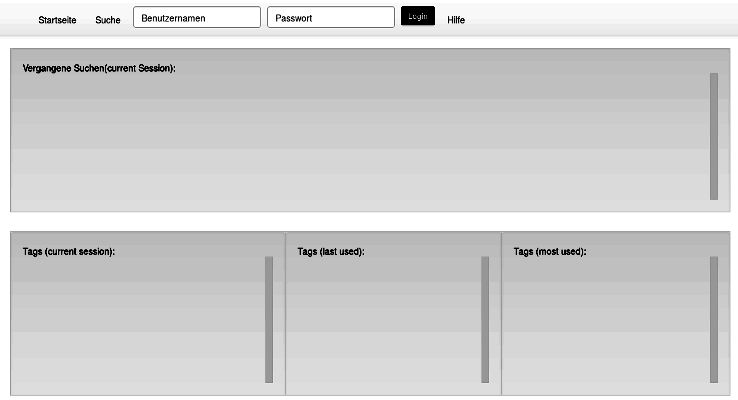
\includegraphics[width=\textwidth]{Masterarbeit_Bilder/www_startseite.png}
    \caption{Startseite der Webanwendung}
    \label{fig:www-start}
\end{figure}  



\begin{figure}[htbp] 
    \centering
    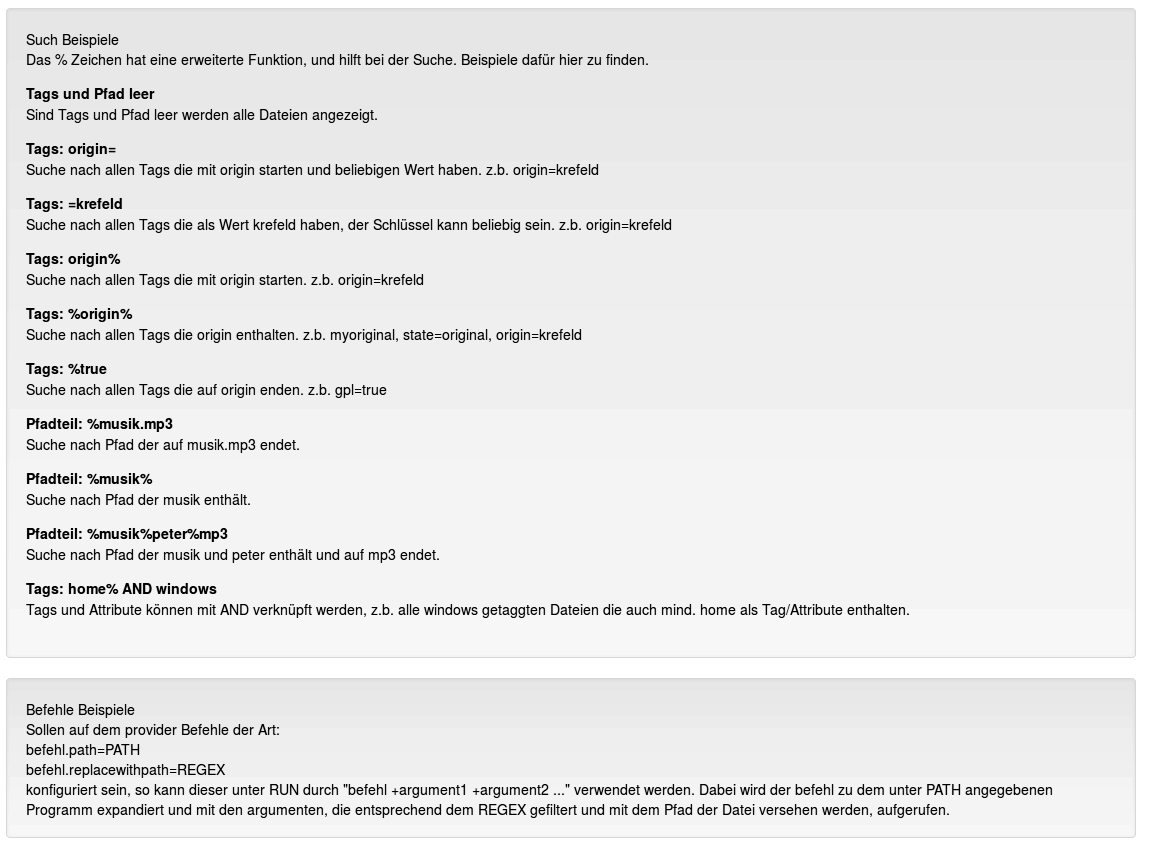
\includegraphics[width=0.8\textwidth]{Masterarbeit_Bilder/www_help.png}
    \caption{Hilfeseite}
    \label{fig:www-help}
\end{figure}  




Es wird kein ,,Faces Flow'' verwendet. Bei Session-Inaktivität wird der auftretende Fehler durch eine konfigurierte Umleitung abgefangen. Ist das Nutzerverhalten evaluiert und fest, ist eine Verwendung der ,,Faces Flow'' API sinnvoller.

Die Abbildung  \ref{fig:www-start} zeigt zudem oben rechts die ,,Hilfe'' an. Auf diese wird auch innerhalb der Anwendung öfter verwiesen. Hier stehen Beispiele und Erklärungen wie Abbildung \ref{fig:www-help} zeigt. 
%% ab hier gehts weiter!!
Da erst nach dem Einloggen alle Funktionen nutzbar sind, sollte der Anwender oben rechts (vgl. Abbildung \ref{fig:www-start}) seinen Benutzernamen und ein Passwort eintragen.
Für den ersten Login werden Administrator-Rechte vergeben. Alle weiteren neuen Anwender bekommen anschließend nur durch diesen Administrator weitere Rechte. Sollte ein Anwender sich das erste Mal am System anmelden, wird automatisch ein Konto angelegt. Sollte das Konto existieren, werden die Identifikationsdaten überprüft und der Anwender bei Erfolg eingeloggt.
Anschließend stehen ihm Konfigurationen und im Fall des Administrator administrative Optionen zur Verfügung.
Die Abbildung \ref{fig:www-einstellungen-admin} zeigt einen eingeloggten Administrator mit leeren Einstellungen und Abbildung \ref{fig:www-einstellungen-user} mögliche Benutzereinstellungen.



\begin{figure}[htbp] 
    \centering
    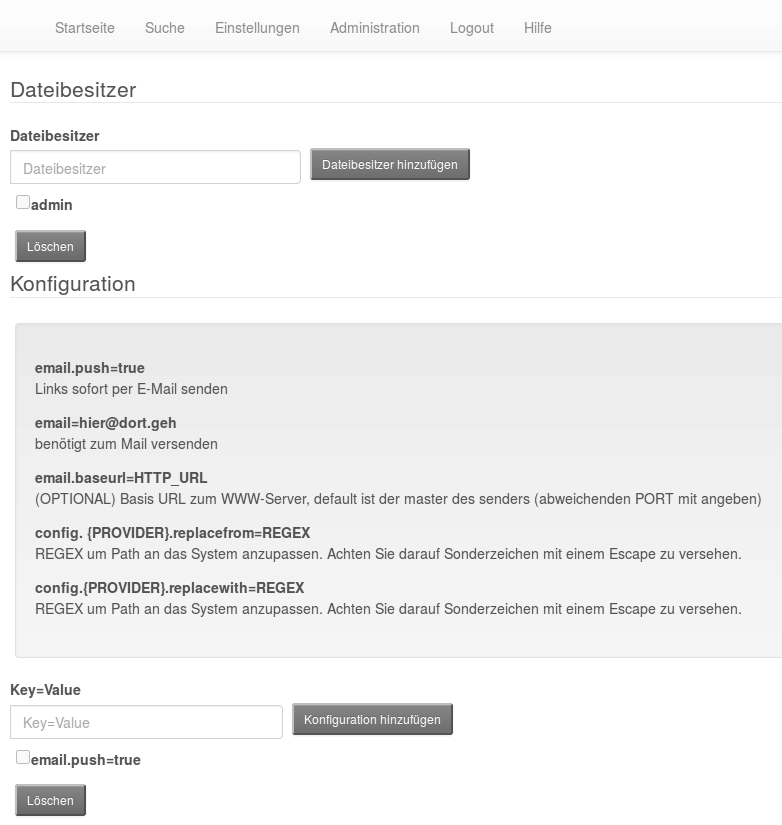
\includegraphics[width=\textwidth]{Masterarbeit_Bilder/www_einstellungen_user.png}
    \caption{Einstellungen eines Anwenders}
    \label{fig:www-einstellungen-user}
\end{figure}  



\begin{figure}[htbp] 
    \centering
    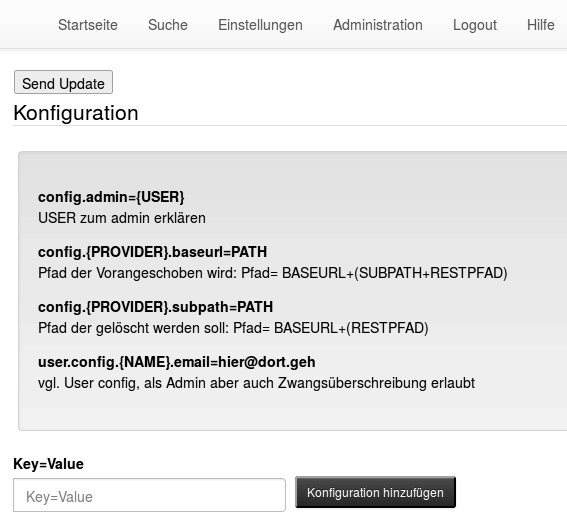
\includegraphics[width=\textwidth]{Masterarbeit_Bilder/www_einstellungen_admin.png}
    \caption{Einstellungen des Administrator}
    \label{fig:www-einstellungen-admin}
\end{figure}  



Nachfolgend gehen alle Szenarien auf die Suche ein, durch einen Klick auf ,,Suchen'' kann dahin navigiert werden. 



\subsubsection{Suche über den Datenbestand}
Die Suchmaske enthält  zwei Eingabefelder, einen Button und eine Ergebnisauflistung, wie in Abbildung \ref{fig:www-suche} zu sehen.
Die in der Analyse angesprochenen Probleme, wie die Plattform übergreifende persistente Speicherung der Schlagworte, ist hier durch Nutzung einer dezentralen Datenspeicherung gelöst. Nutzer verschiedener Plattformen bekommen  für ihre Suche immer die gleiche Oberfläche präsentiert. Um der Plattformunabhängigkeit gerecht zu werden, weichen die Abfragesprache und die Ergebnisauflistung zwischen diesen nicht ab. Die Datenbank legt alle Daten als Zeichenketten ab und beschränkt damit die Suchen auf Mustervergleiche. Dies lässt sich später erweitern und könnte mehr Unterstützung von Vergleichsoperatoren, wie größer oder kleiner sowie ,,Boolesches Retrieval'' bieten \cite{kuhlen2013grundlagen}. Nachfolgende Beispiele beschränken sich allerdings auf Mustervergleiche und erlauben eine Suche nach Dateinamen und eine Suche nach Attributen wie ,,mime-type'' oder ,,Erstellungsdatum''.
Werden Dateipfade und Attribute gleichzeitig gesucht, wie in Abbildung \ref{fig:www-suche2} zu sehen, werden diese durch ein ,,UND'' auf der Datenbank verbunden.



\begin{figure}[htbp] 
    \centering
    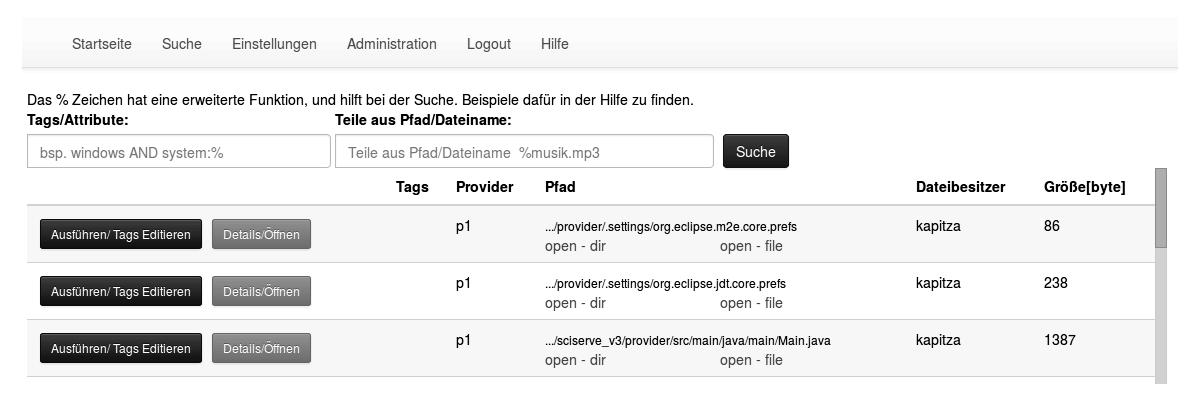
\includegraphics[width=\textwidth]{Masterarbeit_Bilder/www_suche.png}
    \caption{Suchfenster mit leerer Beispielanfrage}
    \label{fig:www-suche}
\end{figure}  

\begin{figure}[htbp] 
    \centering
    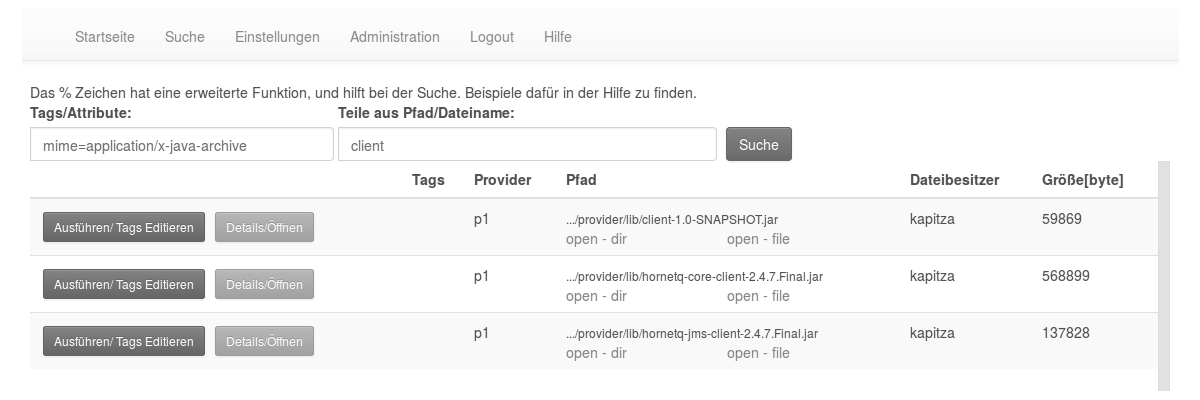
\includegraphics[width=\textwidth]{Masterarbeit_Bilder/www_suche2.png}
    \caption{Suchfenster mit Beispielanfrage nach ,,JAR'' Datei mit ,,client'' im Dateipfad}
    \label{fig:www-suche2}
\end{figure}  

 
\subsubsection{Zugriff auf den Datenbestand}
In diesem Szenario wird gezeigt, wie die Anwendung dem Anwender hilft, auf die im Netzwerk abgelegten Daten zuzugreifen. Wegen der Limitierungen durch den Webbrowser, bedingt durch Sicherheit und nutzbare Funktionen, findet keine Übertragung der Daten statt und auch die direkte Integration ist nur durch Umwege möglich.
Dennoch erfolgt der Zugriff auf die Daten für den Anwender  durch einen vom Betriebssystem bereitgestellten Dateimanager. 
Dazu erkennt die Anwendung anhand des ,,User-Agent'' das Betriebssystem des Anwenders und generiert für dieses ein passendes Script. Dies setzt voraus, dass der Anwender die Netzwerklaufwerke bereits konfiguriert haben.

Ein ,,provider'', beispielsweise mit eindeutigem Namen ,,wichtigedaten'' auf dem Computer ,,server1'' übermittelt alle Meta-Informationen an die Datenbank, nach denen der Anwender suchen kann. Nun kann ein Administrator Standardeinstellungen zum ,,provider'' festlegen. Diese Einstellungen beschreiben die Abbildung der Festplatte des ,,provider'', von der die Daten mit absoluten Pfad kommen, zu den durch eine Netzwerkfreigabe verfügbaren Pfaden.


Anschließende Bilder, beziehen sich auf ein Linux System, die Beschreibungen sind für Windowsanwender.
Die Bilder entstanden anhand der Konfiguration wie in der Abschlussbetrachtung durch die Testumgebung vorgestellt. Als Basis diente dort der Pfad ,,/opt/files'' auf dem Server und ,,/data'' auf dem Endgerät.
Da hier der Dienst SSH verwendet wurde und das Tool ,,sshfs'' entfällt die Angabe eines Server, dies wird beim Verbinden und starten des Tools angegeben.


Für Windows kann eine Datei wie ,,C:\textbackslash{}data\textbackslash{}wichtig\textbackslash{}unterlagen.zip'' auch auf verschiedene Weise freigegeben sein (für Linux vgl. Abbildung \ref{fig:www-orig}).
Die meist nicht zutreffende, einfachste Variante für die Anwendung ist das Freigeben der kompletten Festplatte ,,C:\textbackslash{}'' mit anschließendem Einstellen als Netzwerklaufwerk unter ,,C:\textbackslash{}''.


Es kann auch nur der Unterordner ,,C:\textbackslash{}data\textbackslash{}wichtig'' als Netzwerklaufwerk ,,wichtig'' freigegeben sein. Dann muss vom Administrator der absolute Pfad durch Verwendung von der Konfiguration ,,config.wichtigedaten.subpath=C:\textbackslash{}data\textbackslash{}wichtig'' angepasst werden (für Linux vgl. Abbildung \ref{fig:www-subpath} und das daraus resultierende Ergebnis in Abbildung \ref{fig:www-subpath_0}). Da die Erreichbarkeit so nicht gewährleistet ist, muss ein weiterer Eintrag erfolgen, um den Netzwerkpfad zum ,,provider'' anzugeben. Dies erfolgt durch ,,config.wichtigedaten.baseurl=\textbackslash{}\textbackslash{}server1\textbackslash{}wichtig'' (für Linux mit lokalem ,,mount'' vgl. Abbildung  \ref{fig:www-subpath2}). Das resultierende Ergebnis des Pfades ,,C:\textbackslash{}data\textbackslash{}wichtig\textbackslash{}unterlagen.zip'' erfolgt durch die zwei Konfigurationseinträge dann ,,\textbackslash{}\textbackslash{}server1\textbackslash{}wichtig\textbackslash{}unterlagen.zip'' (für Linux vgl. Abbildung \ref{fig:www-erg}). Da nun aber auch noch ein Anwender auf dem Endgerät ein entsprechender Eintrag zum Verwenden der Freigabe machen kann, unter Windows durch ,,net use'' oder Linux mit ,,mount'', wird ein Pfad auf dem Endgerät z. B. ,,X:\textbackslash{}'' oder unter Linux ,,/other\_mount''  genannt. So können mehr Programme mit den Daten arbeiten. Die gewählte Datei ist auf dem Gerät unter ,,X:\textbackslash{}unterlagen.zip'' erreichbar (für Linux vgl. Abbildung \ref{fig:www-erg2} ).
Dazu kann der Anwender in seinen ,,Einstellungen'' die Konfiguration ,,config.wichtigedaten.replacefrom=\textbackslash{}\textbackslash{}\textbackslash{}\textbackslash{}server1\textbackslash{}\textbackslash{}wichtig'' und ,,config.wichtigedaten.replacewith=X:\textbackslash{}\textbackslash{}'' einstellen  (für Linux vgl. Abbildung \ref{fig:www-subpath3} ). Dabei ist zu beachten, dass ,,reguläre Ausdrücke'' Sonderzeichen interpretieren. 
%%RALF
Die Verdopplung der ,,backslash'' resultieren dadurch. Mehr Informationen können der Java API entnommen werden  \cite{javaregex}.

\begin{figure}[htbp] 
    \centering
    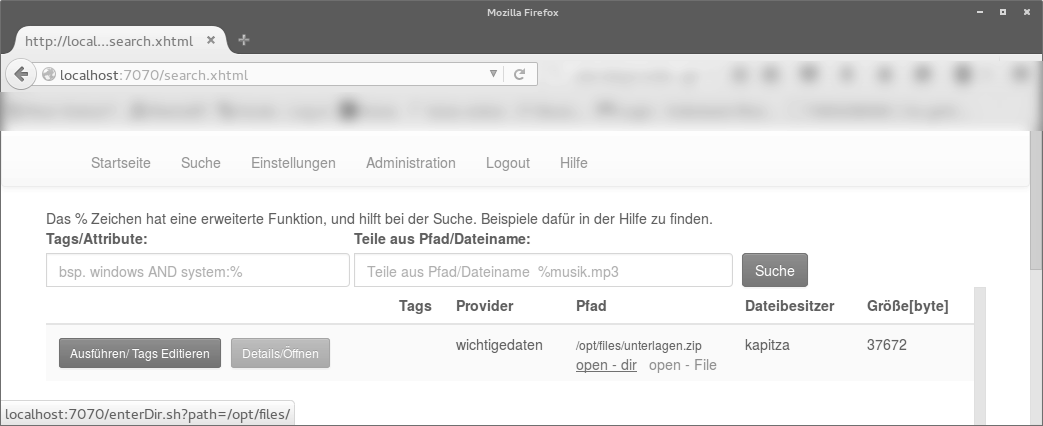
\includegraphics[width=\textwidth]{Masterarbeit_Bilder/original_data_example.png}
    \caption{Ursprüngliche Ausgabe ohne Konfiguration, keine mögliche Nutzung im System, da ,,/opt/files'' nicht existiert.}
    \label{fig:www-orig}
\end{figure}  
\begin{figure}[htbp] 
    \centering
    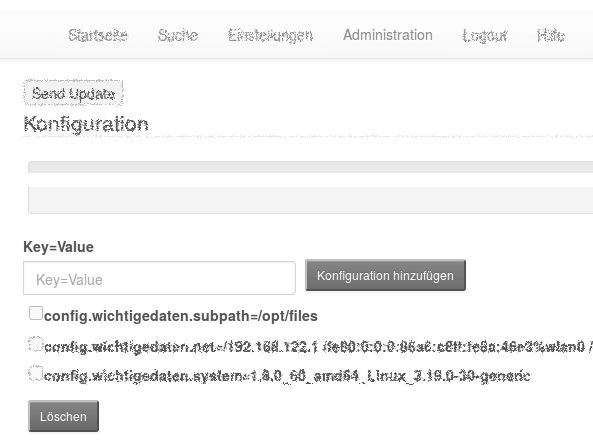
\includegraphics[width=0.8\textwidth]{Masterarbeit_Bilder/admin_remove_sub_cfg.png}
    \caption{Subpath Angabe beim Administrator und löschen von ,,/opt/files'' aus allen Ergebnissen des ,,provider''.}
    \label{fig:www-subpath}
\end{figure}  

\begin{figure}[htbp] 
    \centering
    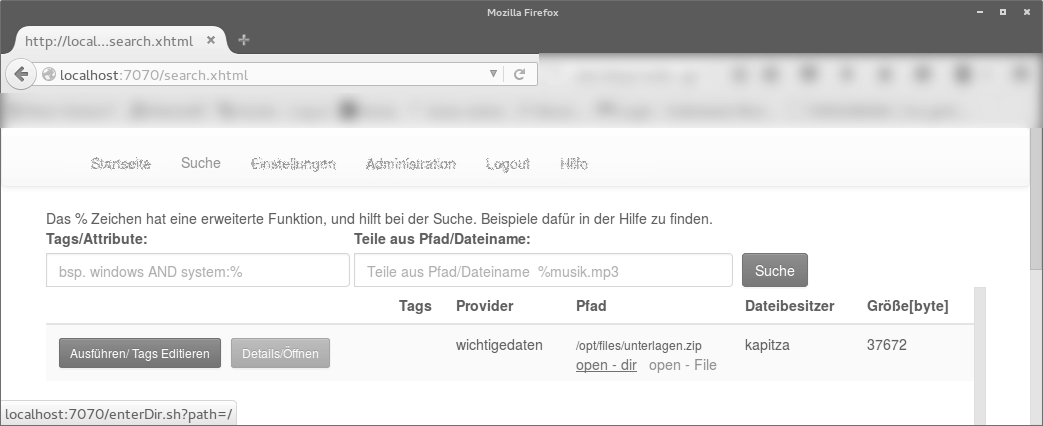
\includegraphics[width=\textwidth]{Masterarbeit_Bilder/admin_remove_sub.png}
    \caption{Ergebnis der ,,subpath'' Angabe beim Administrator nach einer neuen Suche.}
    \label{fig:www-subpath_0}
\end{figure}  
\begin{figure}[htbp] 
    \centering
    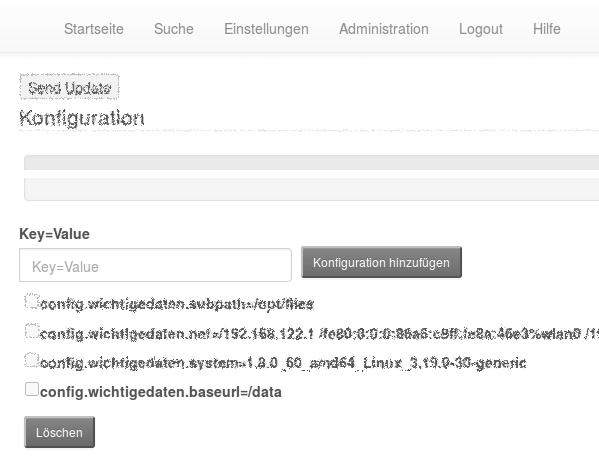
\includegraphics[width=0.8\textwidth]{Masterarbeit_Bilder/admin_change_mount.png}
    \caption{Baseurl Angabe beim Administrator und setzen des PREFIX ,,/data'' auf alle Ergebnisse des ,,provider''.}
    \label{fig:www-subpath2}
\end{figure}  

\begin{figure}[htbp] 
    \centering
    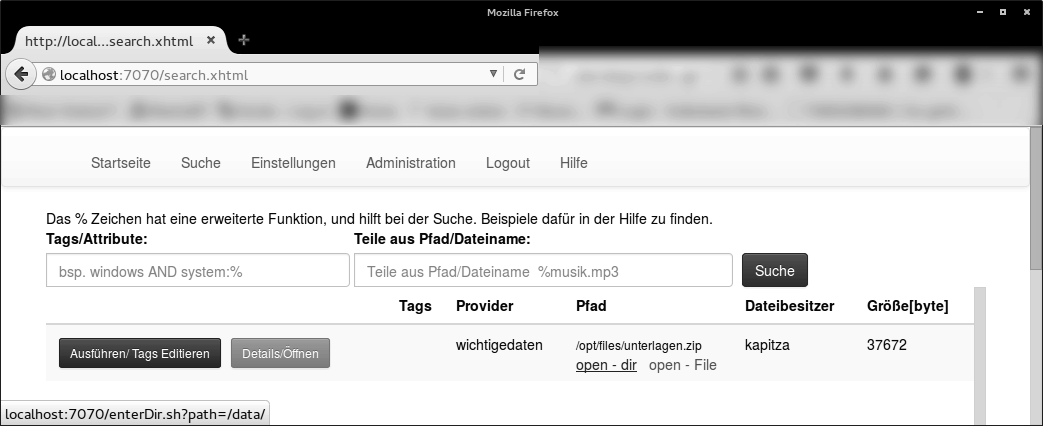
\includegraphics[width=\textwidth]{Masterarbeit_Bilder/open_mount_dir_0.png}
    \caption{Ergebnis der Angaben des Administrator, nach einer neuen Suche.}
    \label{fig:www-erg}
\end{figure}  


\begin{figure}[htbp] 
    \centering
    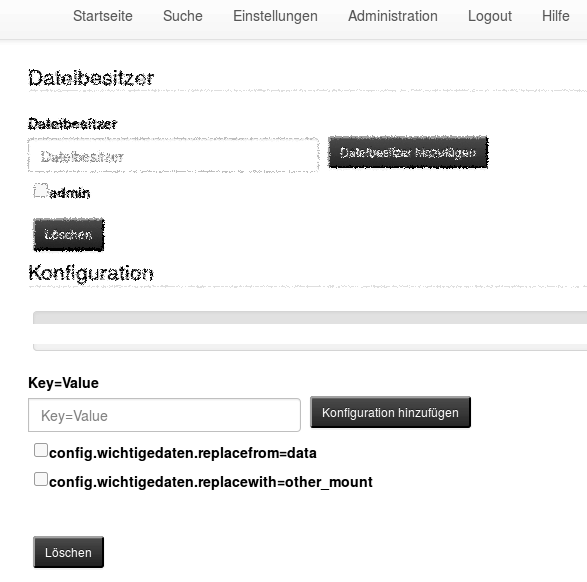
\includegraphics[width=0.8\textwidth]{Masterarbeit_Bilder/user_rewrite_other_mount.png}
    \caption{Neuschreiben der Angaben des Administrator, als Anwender, ,,data'' wird durch ,,other\_mount'' ersetzt. Das System erwartet einen ,,regulären Ausdruck''. }
    \label{fig:www-subpath3}
\end{figure}  

\begin{figure}[htbp] 
    \centering
    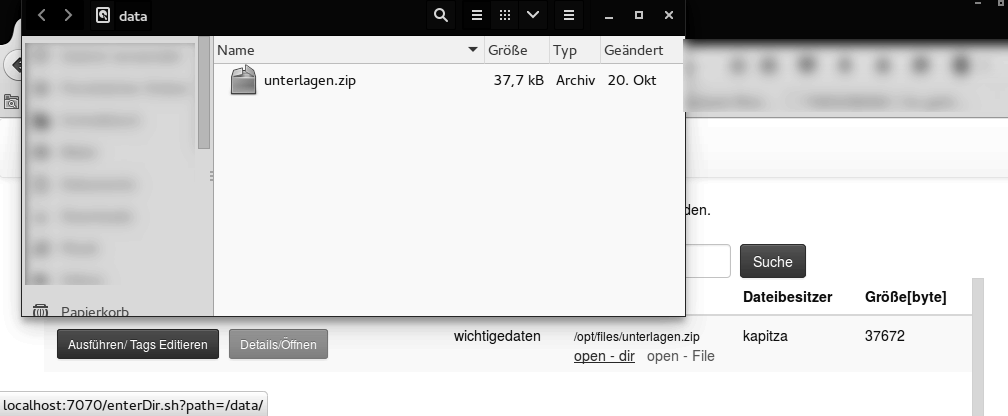
\includegraphics[width=\textwidth]{Masterarbeit_Bilder/open_mount_dir.png}
    \caption{Ergebnis der Angaben des Anwenders, durch Neuschreiben nach einer neuen Suche. Hier ist nach Klicken auf ,,open - dir'' der Dateibrowser ,,nautilus'' im richtigen Ordner geöffnet worden.}
    \label{fig:www-erg2}
\end{figure}  




Da bei den meisten Netzwerken durch den Administrator die Laufwerke festgelegt werden, sollte der durch ihn vorgegebene Standardpfad unter ,,config.{PROVIDER}.baseurl'' für die meisten Anwender ausreichen. Wie der Eintrag dabei aussieht, ist dem Administrator überlassen und könnte auch ,,ftp://SERVER\_FQDN/wichtig'' lauten.
% das gleiche angeben wie OBEN
Die Abbildungen \ref{fig:www-subpath} und \ref{fig:www-subpath2} zeigen die Konfiguration für Linux mit ,,sshfs'' und das daraus resultierende Ergebnis in Abbildung \ref{fig:www-erg}.

Das direkte Arbeiten auf einer Datei bleibt weiterhin dem Betriebssystem überlassen. Die Anwendung hilft durch die generierten Scripte nur beim Navigieren zu den Dateien. Durch einfaches Klicken auf ,,open - dir'' öffnet sich der Dateibrowser auch an entsprechender Stelle. Es bleibt jedoch die Problematik offen, eine Datei vorab zu wählen. Sind die Dateisammlungen groß, muss der Anwender im Fenster dennoch nach dem richtigen Dateinamen suchen. Geht es lediglich um ein ,,Öffnen'' der Datei mit einer Standardanwendung, sollten ein ,,open - file'' ausreichen und das generierte Script öffnet die Datei mit der hinterlegten Anwendung.
%% ralf?
Weiterführende Integration sowie ein Vermeiden von Scripten, die der Anwender auch erst ausführen muss, was nach einmaliger Einstellung weniger störend ist, erfordert ein Addon im Browser oder aber eine Anwendung auf dem Endgerät. Es ist in HTML nicht möglich, bestimmte Standardanwendungen in der Weboberfläche zu verwenden. Dies wäre gerade für eine Dateiverwaltung hilfreich.

 
\subsubsection{Synchronisation der Daten}
Dieses Szenario wird von dieser Anwendung kaum unterstützt. Es ist einzig die Möglichkeit gegeben zwischen zwei Peers Dateien auszutauschen, indem der internen ,,publish'' Befehl freigegeben wird. Jedoch erfordert es immer noch das Eingreifen eines Anwender, der die Datei erst noch veröffentlichen muss. Durch Eintippen von ,,publish'', wie in Abbildung \ref{fig:www-cmd-pub} zu sehen, wird die entsprechende Datei auf alle angemeldeten ,,provider'' verteilt.

\begin{figure}[htbp] 
    \centering
    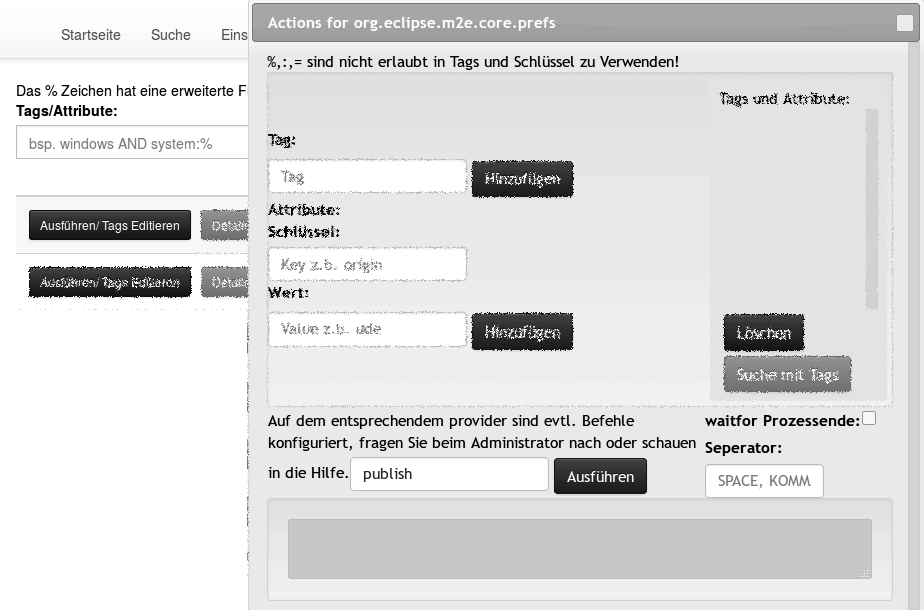
\includegraphics[width=\textwidth]{Masterarbeit_Bilder/www_cmd_publish.png}
    \caption{ ,,publish'' Befehl auf dem ,,provider'' auslösen. Der Empfänger meldet sich nach entsprechender Nachricht des  ,,provider'' direkt um einen Dateiaustausch zu starten. Beim Melden überträgt der Empfänger seine Verbindungsinformationen.}
    \label{fig:www-cmd-pub}
\end{figure}  

\bigskip

Hier bedarf es noch einiges an Arbeitszeit, um einen einfachen Synchronisationsmechanismus zu erstellen, wie er von Diensten wie ,,Dropbox'' oder ,,Google Drive'' bekannt ist.

 
\chapter{Abschlussbetrachtung}
 
\chapmd{Projektmanagementkurs Universität Duisburg-Essen}{,,Ich will, dass Sie so gut werden, dass es mich meinen Job kostet.''}


Nachfolgend wird ein Testaufbau beschreiben und auftretende Probleme diskutiert. Der Versuchsaufbau bezieht sich nachfolgend auf Linux Systeme und umfasst einen Client, der via Webbrowser die ,,www'' Anwendung bedient und eine Weboberfläche zum Mailen verwendet.
Die Testumgebung besteht aus zwei Server und einem Client. Der zweite Server wird extern verwaltet und ist lediglich für E-Mail zuständig. Das Einrichten und Verwalten eines Mailserver wird hier nicht berücksichtigt. Es wird davon ausgegangen, dass eine gültige E-Mail-Adresse mit passendem Benutzer-Account existieren, um dem Peer ,,database'' den nötigen Zugriff zu ermöglichen. Eine weitere Annahme ist, dass der Mailserver ohne Probleme durch die Firewall erreicht werden kann.

Einen Datenserver mit Netzwerknamen ,,fileserver'' dessen Daten unter ,,/opt/files'' liegen, wird durch ,,sshfs'' am Client unter dem Pfad ,,/data'' gemountet.

Der Datenserver und Client sind im LAN betreiben und nicht durch eine Firewall explizit gesichert. Auf dem Datenserver ist Java 8 installiert und es werden als Dienste nur ,,ssh'' sowie die in der Arbeit beschriebenen Projekte wie ,,database'', ,,www'', ,,master'', ,,provider'' ausgeführt. Da der ,,master'' eingebettet bereits ,,database'' und ,,www'' startet, muss im verwendeten Speicherort nur noch der ,,provider'' gestartet werden, um die Analyse für  dort liegende Dateien zu starten und überwachen.

Das Starten erfolgt mit einfachen Befehlen in der Konsole. Unter Windows reicht i. d. R. ein Doppelklick, um mit Standardwerten die Anwendung auszuführen. 

\bigskip

Starten des ,,master'' mit: 
\begin{quote}
    cd /PATH\_TO\_DOWNLOAD\_DIR/ \\
    unzip master-VERSION.zip \\
    cd master \\
    java -jar master-VERSION.jar 
\end{quote}

Die Konfiguration wird aus der Datei ,,server.properties'' gelesen und beinhaltet das Geheimnis, die Konfiguration für E-Mail und Webanwendung.

\bigskip

Der ,,provider'' wird mit:
\begin{quote}
    
    cd /PATH\_TO\_DOWNLOAD\_DIR/ \\
    unzip provider-VERSION.zip \\
    cd provider \\
    Allgemein: java -jar provider-VERSION.jar (provider.properties WATCH\_DIRS ...)\\
    Beispiel: java -jar provider-VERSION.jar provider.properties /opt/files
\end{quote}

gestartet. Es ist beim Start möglich, die Konfiguration der Ordner mitzugeben. Dazu muss die Konfigurationsdatei für Kommunikation und Dienst sowie eine Liste von Ordner angegeben werden. Ist kein Parameter gegeben, wird der Standard mit ,,provider.properties'' und als zu beobachtender Ordner der aktuelle Pfad, hier ,,/PATH\_TO\_DOWNLOAD\_DIR/provider'', angenommen.


Dadurch sind auf dem Server alle Dienste bereitgestellt. Auf dem Client wird das Laufwerk mit ,,sshfs user@fileserver:/opt/files /data'' eingebunden.

Ein Zugriff auf die Weboberfläche liefert jedoch nicht das gewünschte Ergebnis (Abbildung \ref{fig:www-orig}). Durch eine administrative Einstellung wird nun der Pfad geändert. In Abbildungen \ref{fig:www-subpath} und \ref{fig:www-subpath2} als Administrator global oder durch den Anwender vgl. Abbildung \ref{fig:www-subpath3}. Das Ergebnis ist in beiden Fällen gleich und in Abbildung \ref{fig:www-erg} zu sehen.



\section{Probleme und Schwächen}

Bei der Anwendung sind einige Funktionen wie die Integration in den Desktop nur über Umwege realisierbar gewesen.
,,Einen Schraubendreher nutzen um einen Nagel zu versenken'' wie es nicht treffender sein könnte \cite{cederholm2009web}. Die Integration lässt sich jedoch nicht anders realisieren. Deswegen ist festzuhalten, dass eine solche Anwendung nicht ohne Addons im Webbrowser vernünftig umsetzbar ist. Da jedoch zu viele verschiedene Webbrowser existieren, ist die Realisierung durch eine separate Client-Anwendung sinnvoller.

In dem erzeugten \acrshort{p2p}-Netzwerk wird davon ausgegangen, dass sich die Peers untereinander vertrauen und sich alle Peers regelkonform verhalten, da bei der Kommunikation, auch wenn mit mehrfachen Antworten gerechnet werden muss, sonst falsche Informationen den Fragen zugeordnet werden.

Da in den meisten Dateisystemen Sonderzeichen als Dateinamen verboten sind, wurde hier nicht beachtet, dass ein Script als Dateinamen Kodiert auf einem Client ausgeführt werden könnte \cite{winforbit}. Sollten Dateien einen Namen wie \verb|<script>alert('bad javascript')</script>| existieren, dann könnte an einigen Stellen im Code von ,,www'' dieses auch im Webbrowser ausgeführt werden. Da diese Fälle nur künstlich erzeugt werden können, blieb dieses Problem unbeachtet.

Auch das Herausfinden der Existenz einer Datei ist auf einem Peer nicht effizient gelöst worden.
Es wird für jede Datei im Betriebssystem nachgefragt. Dafür wird von der Festplatte gelesen.
Schneller feststellen, ob eine Datei nicht existiert, könnte bei den Peers durch ,,Bloom Filter'' realisiert werden. Dies würde die Festplatte nicht unnötig  zum Anlaufen bringen, um festzustellen, dass die Datei nicht vorhanden ist. Da für ein definitives Ja dennoch auf die Platte geschaut werden muss, sollte ein Cache in zweiter Ebene und erst als letzte Möglichkeit der Plattenzugriff erfolgen \cite{bejeck2013getting}.  

Fehlerhafte Programme, die beim Ändern einer Datei diese löschen und komplett neu schreiben, können den ,,provider'' behindern und dafür sorgen, dass die Prüfsummen der Datei neu berechnet werden. Bei den angenommenen Dateigrößen ist das nicht wünschenswert, der Fehler lässt sich aber nicht durch das Programm selbst erkennen. Programme, die das Änderungsdatum aktualisieren gehören ebenso dazu, da die Prüfsumme und Datum stark zusammenhängen.

Probleme beim Speichern von Prüfsummen haben im Test gezeigt, dass stillschweigend die alten Attribute mit den neuen überschrieben werden, wenn der Speicherplatz für diese nicht ausreicht. Daher wurde die Limitierung auf wenige Variablen und Attribute in den Dateien gemacht. Gerade Linux ist anfällig für dieses Verhalten.
Ein Ansatz mit beschreibenden Dateien im separaten oder gleichen Ordner ist genauso schwer zu verwalten wie eine gleichnamige versteckte Datei, da hier Fehler durch Umbenennen, Verschieben und Kopieren die entsprechende andere Datei nicht beachtet. Einen ,,Watch Service'' dafür zu implementieren, wäre umständlich und könnte Datenbestände niemals zuverlässig zusammenführen.

Das Projekt ,,bridge'' wurde nicht ausreichend genug getestet und kann noch sehr viele Probleme beinhalten. Es ist daher mehr als Konzept zu werten. Zu den nicht getesteten Problemen gehören Zyklenerkennung sowie doppelte Nachrichten. Ein \acrshort{ttl} ist zwar prinzipiell eine Möglichkeit, beschränkt aber das Skalieren der Systeme.

Der Speicherverbrauch wird größer durch die Verwendung von Hash-Tabellen. Eine einfache Liste ist im Test zu langsam gewesen und würde bereits bei kleinen Datenbeständen die Festplatte unnötig oft stoppen und neu anlaufen lassen. Die heutigen Computer können der Anwendung die 256 MB Speicher zusichern und mit entsprechenden Java Optionen im System gesetzt werden.

Auch wenn die Anwendung portabel und betriebssystemunabhängig ist, sind die gelieferten Dateipfade durch Kodierungen und Zeichen nicht unabhängig. Es bedarf daher immer das Eingreifen des Anwender, um durch ,,reguläre Ausdrücke'' den korrekten Pfad für das Endgerät zu erzeugen.

Durch die verwendeten Bibliotheken sind einige Probleme entstanden, die durch ein Update der Bibliothek später evtl. behoben werden. Darunter ist eine ,,OutOfMemory-Exception'', die vom \acrshort{jms} erzeugt wird, weil die verwendete Pufferung nicht freigegeben wird. Das Auftreten scheint jedoch mit ,,Hibernate-to-Ram'' zusammenzuhängen. 

Kleinere Fehler in den neuen Funktionen von Java 8 wie beim Arbeiten mit Streams und paralleler Verarbeitung wurden durch entsprechende Java 7 Logik ersetzt. Da Java 8 noch neu ist, kommen viele Bibliotheken nicht mit der neuen API klar, so dass WELD als CDI-Umgebung und \acrshort{jpa} nur mit Java 7 Code ausgeführt werden kann.

Eine Eigenart beim \acrshort{orm} durch das ,,ManyToMany'' und den Gebrauch von Join-Tabellen  erlaubte kein einfaches Löschen ohne weiteres Anlegen von Klassen. Es wurde hier auf eine ,,Embedded Collection'' umgestellt. Daher ist jedoch in den entsprechenden Tabellen nicht Prüfsumme der Fremdschlüssel, sondern die ID der Datei. Das Problem der Zuordnung wurde dadurch in der Anwendung realisiert, jedoch sind die Tabellen nicht ,,normalisiert''.

Das \acrshort{jpa}  erlaubt ,,lazy-loading'', welches in dieser Anwendung explizit  abgestellt wurde.
Der Grund dafür ist, dass bei einer Datenübertragung im \acrshort{jms}  kein Nachladen der fehlenden Informationen erfolgte. Ob dies mit Java 8 zusammen hängt oder aufgrund des eingebetteten Modus wurde nicht evaluiert. Als Lösung wurde der ,,EAGER'' Modus bei den Schlagworten und Hash-Listen verwendet.

Einschränkungen des eingebetteten Modus sind zudem mangelnde Unterstützung von Validierungen durch Notationen sowie einige API im JSF und \acrshort{cdi} Umfeld.
Hier scheint das Problem in der verwendeten Version des Anwendungsserver zu sein. Im eingebetteten Modus werden von diesem nicht alle API geladen und anders konfiguriert als in der typischen Installation. Kurz vor Ende der Arbeit wurde jedoch ein Update angekündigt, es bleibt dem Anwender überlassen, das Update zu nutzen.


Windows als ,,provider'' hat durch installierte Firewall und Virenscanner im Test gezeigt, dass Fehler nicht angezeigt werden. Die Software war nicht ohne administratives Handeln in der Lage, einen Port zur Kommunikation zu öffnen. Ob dies durch eigenes Einstellen oder das Standardverhalten ist, wurde nicht weiter überprüft. Der Kommunikationsport muss neben dem festlegen in der Konfigurationsdatei auch auf dem Betriebssystem und ggf. im Virenscanner entsprechend eingestellt werden. Das bekannte Benachrichtigungsfenster scheint hier nicht mehr zu existieren. Die zweite Firewall mit  \acrshort{nat} ist hier noch nicht aktiv und muss danach auch noch überwunden werden. Unauffälliger ist dabei noch die höhere CPU-Last, da Windows viel zu viele Events liefert bei der Dateiüberwachung, welche erst durch den selbst geschriebenen Service reduziert werden.

Beim Erstellen der Weboberfläche ist in heutigen Anwendungen ,,ajax'' in Verwendung. Jedoch ist bei Verwendung von Formularen ein Fehler in JSF, welcher durch ein angepasstes Javascript erst behoben wurde. 


\subsection{Mac OS und der Webbrowser}
Nach einigen Tests auf einem Mac OS Rechner, konnte festgestellt werden, dass das Ausführen der Scriptes, welches von der ,,www''-Anwendung generiert wird nicht automatisch zur Ausführung konfiguriert werden konnte. Die Sicherheitseinstellungen sind anders als in Linux oder Windows mit normalem Anwenderwissen nicht umzustellen.
Es bleibt nur der ,,Workaround'' (vgl. Abbildung \ref{fig:apple}) durch öffnen eines Terminal welches die gespeicherten Scripte ausführt.
\begin{figure}[htbp] 
    \centering
    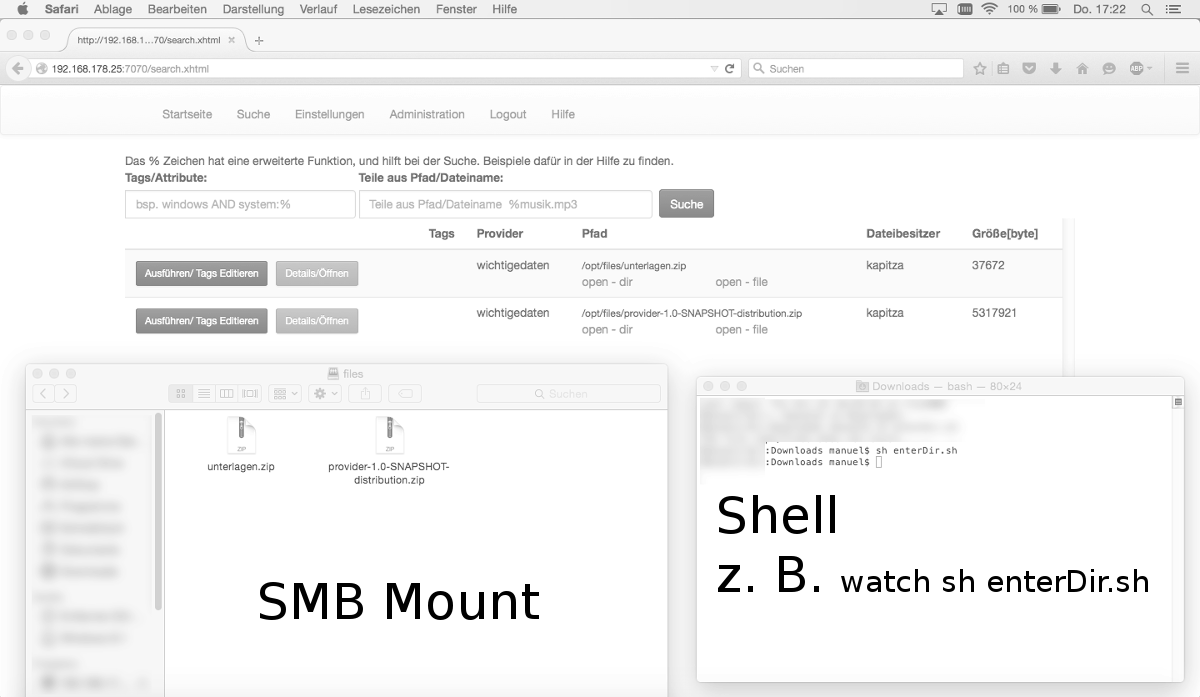
\includegraphics[width=0.8\textwidth]{Masterarbeit_Bilder/appel_terminal.png}
    \caption{Mac OS, Konfigurierter SMB mount ,,files'' der durch das Terminal geöffnet wird. }
    \label{fig:apple}
\end{figure}  

Eine Automatisierungshilfe könnte das Nutzen des ,,watch'' Befehls sein. Dieser kann mit ,,brew'' oder ,,port'' installiert werden. 
Eine Simulationsannäherung wäre durch \verb|while :; do clear; your_command; sleep 2; done| gegeben.
Als Befehl würde die gespeicherte Datei in Downloads ausgeführt werden. Das wäre Beispielsweise mit \verb|watch enter.sh| möglich.
Ein automatisches Speichern ist in Safari und Firefox schnell einzustellen.


 
 

\section{Zusammenfassung und Ergebnis}
Zum Reflektieren der Anforderungen werden diese der aktuellen Realisierung gegenübergestellt.


\begin{itemize}
	\item Zuordnung einer Person zu den diversen Konten und zu einer Datei als Besitzer/ Verantwortlicher\\
	Diese Aufgabe muss durch den Anwender über eine entsprechende Oberfläche gemacht werden. Die Zuordnung als Dateibesitzer kann in den Einstellungen -- wie in Abbildung \ref{fig:app-cfg-datei} zu sehen ist -- gemacht werden. Nötige Informationen  stammen vom ,,provider'' und ausgewählte Daten werden in den ,,database''-Peers gespeichert.
	
	\item Auslesen der Informationen einer Datei unter Beachtung des Dateisystems \\
	Durch das Java NIO werden das Auslesen und auch die Überwachung der Änderungen im Dateisystem bereitgestellt.
    Eine Implementierung ist im ,,provider'' realisiert.

    \item Anzeigenanpassung und individuelle Unterstützung je nach verwendeter Plattform \\
	Das JSF sowie die verwendeten HTML5-Elemente sind Grundlage der Anzeigen und bedürfen keiner Anpassung. Für die Integration wird entsprechend der Plattform ein Script generiert.
	\item Übertragung der Dateien zwischen den DMS\\
   Diese wird nicht direkt ersichtlich  vom System unterstützt. Eine Freigabe und Übertragung ist durch den ,,publish'' Befehl möglich, jedoch kann durch Firewalls die Kommunikation nicht garantiert werden.  
	\item Benachrichtigung über den Vorgang einer Datei\\
	Das System versendet eine E-Mail an den hinterlegten Besitzer der Datei. Sollte keine Mailadresse bekannt sein, entfällt diese Funktion. Diese Funktion ist in der ,,database'' implementiert.
	\item Persistente Speicherung auch der Attribute, die nicht vom Dateisystem unterstützt werden\\
	Es wird eine Datenbank verwendet, um Attribute systemübergreifend zu speichern.
    Die einzigen, welche in den ,,erweiterten Attributen'' gespeichert werden, sind die Prüfsumme und deren Erzeugungsdatum. Um konkurrierende Zugriffe zu vermeiden wird ein drittes als Sperre verwendet. Der Grund für die begrenzte Speicherung liegt in der noch immer, gerade unter Linux, schlechten Systemunterstützung.

    Im Dateisystem kann je nach Plattform nachgesehen werden, ob zu einer Datei die Prüfsummen berechnet wurden:
    \begin{itemize}
        \item Windows mit \verb|dir /r|
        \item Linux mit \verb|attr -l|
        \item Mac OS mit \verb|xattr|
    \end{itemize}
    
    und der entsprechenden Datei als Parameter.
    
	\item Verlinken der DMS \\
    Ein Konzept ist mit der ,,bridge'' beschreiben worden.
	\item Erkennung doppelter Dateien\\
Durch die Oberfläche lässt sich nach Prüfsummen suchen, aktuell werden Tags so an jedes Duplikat gehangen. Eine spezielle Oberfläche muss jedoch noch realisiert werden.
\end{itemize}



\section{Diskussion und Ausblick}
Diese Anwendung unterstützt hinsichtlich der Aufgabenstellung die Suche.
Aus zeitlichen Gründen ist die Dateisynchronisierung nicht so weit gekommen, dass diese durch den Anwenden intuitiv nutzbar ist. Wegen der Verwendung von HTTP ist es nicht möglich große Datenmengen zu transportieren, deshalb muss ein weiterer separater Dienst erstellt werden. Eine Möglichkeit wäre, die Realisierung durch eine Implementierung eines SSH-Dienstes, welcher Transfer, Tunnelaufbau und Befehlsausführung realisiert. 

Gedanklich wurde jedoch beachtet, dass ein Übertragen ähnliche Dateien berücksichtigen muss, um Verschiebungen zu erkennen und dadurch nicht neu zu übertragen. Das erfordert jedoch ein verzögertes Löschen. Die Nutzung externer Befehle macht das Programm sehr flexibel und Analysen vom ,,provider'' durch das Nutzen von Apache Tika, wie in der Einleitung \ref{chap:einleitung} erwähnt, verfeinert werden. Diese Bibliothek kann jedoch nicht alle Dateitypen erkennen.
Auch die ,,database'' lässt sich erweitern und durch \href{http://lucene.apache.org/solr/}{ Apache Solr}
besser indizieren. Die Integration lässt sich aber erst realisieren, wenn die Datenstruktur feststeht, da der Aufbau des Index und der Anfragen nicht ständig geändert werden kann. Die Flexibilität einer Datenbank hat Apache Solr nicht.

OSGI ist als Schlagwort im Java-Umfeld immer wieder zu finden. Das macht die Anwendungen jedoch nicht so einfach paketierbar und eine eingebettete Version kann dadurch sehr schnell komplex werden. Auch ist mehr Verwaltung zu Beginn nötig, was das Entwickeln verlangsamt. Zudem ist der ,,overhead'' bei kleinen Anwendungen durch die nötigen Dienste zu groß.

\subsection{Version 2.0}
Wie oben bereits angesprochen, ist ein SSH-Dienst sehr flexibel. Die Integration des Dienstes in die Anwendung würde ein Vermitteln zwischen den Peers durch Tunnel vereinfachen. Die Kommunikation könnte vom \acrshort{jms} auf die Kontrollverbindung des SSH umgestellt werden und würde durch Zertifikate die Sicherheit in der Kommunikation und Authentifizierung bringen. Beim Vermitteln würde das Mitlesen der Daten nicht möglich sein, sofern die betroffenen Peers ihre Fingerprints zuvor ausgetauscht haben.

Dieser Ansatz wurde in ,,Version 1.0'' nicht verfolgt, weil die Generierung von Schlüsseln komplex ist und es noch keine einfache Möglichkeit gibt, im Programmcode dies in vorgegebener Zeit zu automatisieren.
Es existieren eine menge Bibliotheken für SSH, jedoch nur wenige, die auch einen Server implementiert haben.
SSH besteht aus mehreren Diensten und die getesteten Bibliotheken wie ,,Apache SSHD'', unterstützen diese Dienste nicht umfänglich genug, um damit eine Anwendung zu realisieren.

Die meisten Bibliotheken verbinden sich auf Linux Server, was den Anforderungen, Plattform unabhängig zu sein widerspricht. Es existieren zwar viele Portierungen des Openssh-Server, jedoch binden gerade unter Linux diese Dienste an das Betriebssystem an und lassen sich nur schwerlich für die Anwendung nutzen, ohne komplexe Konfigurationen zu erstellen.

\subsection{Entwicklung}
Das Projekt wird in der Freizeit weiterentwickelt und befindet sich auf Github:\\
 \verb|https://github.com/JensKapitza/sciserver| \\ 
Interessierte können dort gerne mit mir Kontakt aufnehmen.

Die CD beinhaltet:
\begin{itemize}
    \item \LaTeX - Code, Java Code [keine Bibliotheken die durch Maven installierbar sind], Java Distribution ZIP (,,master''-Peer und ,,provider''-Peer die das Ausführen der Anwendung ermöglichen)
\end{itemize}



% Anhang
\appendix
\cleardoublepage{}


\printindex
\printglossaries


% Literaturverzeichnis
\backmatter{}

% Sprache für Literaturverzeichnis wählen
%\nocite{de}
%\nocite{en}
%teilweise verändert, aus der Webseite: 
% http://www.is.uni-due.de/lehre/bachelor_und_masterarbeiten/aufbau_einer_abschlussarbeit/
% 
\bibliographystyle{Formatvorlage_IS}
%\bibliographystyle{apalike}
\bibliography{books}



\end{document}